%&latexf
\documentclass[11pt,a4paper]{article}
\usepackage{color}
\setlength{\hoffset}{-0.5in}\hoffset-0.5in
\setlength{\textwidth}{15cm}
\usepackage{hyperref}
\usepackage{amsmath, amsfonts, amsthm, amssymb}
\usepackage{verbatim}
\usepackage{stmaryrd}
\usepackage{fancyhdr}
\usepackage{color}
%\usepackage{graphicx}
\usepackage{float}
%\usepackage[demo]{graphicx}
%\usepackage{subfigure}
\usepackage{caption}
%\usepackage{subcaption}
\usepackage{booktabs}
\usepackage{multirow}
\usepackage{rotating}
\usepackage{tikz}
\usetikzlibrary{positioning}
\usetikzlibrary{arrows}

\linespread{1.5}
%\font\twelvemsb=msbm10 at 12pt
\newfam\msbfam
%\textfont\msbfam=\twelvemsb
\def\Bbb#1{\fam\msbfam\relax#1}

\topmargin = 20pt
\voffset = -20pt
\addtolength{\textheight}{2.0cm}
\newtheorem{theorem}{Theorem}[section]
\newtheorem{exa}{Example}[section]
\newtheorem{corollary}[theorem]{Corollary}
\newtheorem{lemma}[theorem]{Lemma}
\newtheorem{proposition}[theorem]{Proposition}

\theoremstyle{definition}
\newtheorem{definition}[theorem]{Definition}
\newtheorem{remark}[theorem]{Remark}
\newtheorem{notation}[theorem]{Notation}
\newtheorem{assumption}[theorem]{Assumption}
\newtheorem{conjecture}[theorem]{Conjecture}

\newcommand{\ind}{1\hspace{-2.1mm}{1}} %Indicator Function
\newcommand{\I}{\mathtt{i}}
\newcommand{\D}{\mathrm{d}}
\newcommand{\F}{\mathrm{F}}
\newcommand{\E}{\mathrm{e}}
\newcommand{\GP}{\mathcal{GP}}
\newcommand{\EE}{\mathbb{E}}
\newcommand{\RR}{\mathbb{R}}
\newcommand{\sgn}{\mathrm{sgn}}
\newcommand{\atanh}{\mathrm{arctanh}}
\def\equalDistrib{\,{\buildrel \Delta \over =}\,}
\numberwithin{equation}{section}
\def\blue#1{\textcolor{blue}{#1}}
\def\red#1{\textcolor{red}{#1}}

\setlength{\parindent}{2em}
\setlength{\parskip}{1em}
\let\vec\mathbf

\begin{document}
	%The following commands include several pages which contain the front page, acknowledgements,...
	\thispagestyle{empty}
\null\vskip0.2in%
\begin{center}
\LARGE{{\bf 
GAUSSIAN PROCESS REGRESSION \\-- A MACHINE LEARNING APPROACH TO DERIVATIVE PRICING}}
\end{center}

\vspace{0.5cm}

\begin{center}
{\Large {\bf by}}\\
\mbox{} \\
{\Large {\bf Haibo Li (CID: 01441128)}}
\end{center}

\vspace{1.5cm}

\begin{center}
\large{\bf{Department of Mathematics \\ Imperial College London \\
London SW7 2AZ \\ United Kingdom}}
\end{center}



\vspace{5.5cm}

\begin{center}
\large{\bf{Thesis submitted as part of the requirements for the award of the \\
MSc in Mathematics and Finance, Imperial College London, 2017-2018}}
\end{center}

\vspace{2cm}


	%\thispagestyle{empty}


\mbox{}\newline\vspace{10mm} \mbox{}\LARGE
%
{\bf Declaration} \normalsize \vspace{5mm}

The work contained in this thesis is my own work unless otherwise stated.

\bigskip
\bigskip
\bigskip


Signature and date: 

Haibo Li

11/09/2018

\newpage

\mbox{}\newline\vspace{10mm} \mbox{}\LARGE
%
{\bf Acknowledgements} \normalsize \vspace{5mm}

I would like to thank my supervisor at Imperial College, Dr. Thomas Cass for his constant help and support, as well as for his insightful suggestions.

I would also like to thank my manager at Citigroup, Karim Berradi for giving me the opportunity to do this Placement project on his team. I am most grateful to his help and numerous inspirational guidance during the past three months.

I also want to thank other members on the team: H\aa vard Sandvik, Nikos Karantzoulis, Stephane Guilherme Gomes, Mohamed Boualam, He Ren and Yacine Debbabi for their help in many aspects which made the past three months a very pleasant experience.







	
	%%%
	\setcounter{tocdepth}{4}
	%%%
	
	\tableofcontents %% This includes the table of contents, which is organised automatically, 
	%% and used your section / subsection.
	
	\newpage %%This simply means that the next part of text will start on a new page.
	
	%%%%%%%%%%%%%%%%%%%%%%%%%%%%%%%%%%%%%%%%%%%%%%%%%%%%
	\fancyhead{}
	\fancyfoot{}
	\pagestyle{fancy} 
	\fancyhead[RO,LE]{\sffamily\small \thepage}
	\fancyhead[LO,RE]{\sffamily\small \nouppercase{\rightmark}}
	\renewcommand{\headrulewidth}{0.35pt}
	\renewcommand{\footrulewidth}{0.0pt}
	%%%%%%%%%%%%%%%%%%%%%%%%%%%%%%%%%%%%%%%%%%%%%%%%%%%%
	
	
	
	
	
	%%%%%%%%%%%%%%%%%%%%%%%%%%%%%%%%%%%%%%%%%%%%%%%%%%%%
	%%%%%%%%%%%%%%%%%%%%%%%%%%%%%%%%%%%%%%%%%%%%%%%%%%%%
	%%%%%%%%%%%%%%%%%%%%%%%%%%%%%%%%%%%%%%%%%%%%%%%%%%%%
	%%%%%%%%%%%%%%%%%%%%%%%%%%%%%%%%%%%%%%%%%%%%%%%%%%%%
	%%%%%%%%%%%%%%%%%%%%%%%%%%%%%%%%%%%%%%%%%%%%%%%%%%%%
	%%%%%%%%%%%%%%%%%%%%%%%%%%%%%%%%%%%%%%%%%%%%%%%%%%%%
	\section{Introduction}
	One of the challenges in financial derivatives pricing is calibrating curves from market data and running a large number of Monte Carlo simulations to price more exotic products. This process is usually very time consuming especially when a  structured product with a lot of underlyings is priced. One way to tackle this problem  is using a trained machine learning model to replicate the price without doing all the calibrating and simulations. In this paper, one class of regression model, the Gaussian Process Regression(GPR) is investigated for replicating the price of one particular structured product, namely Synthetic Collateralized Debt Obligation.
	
	\subsection{CDS, CDD and Synthetic CDO}
	The focus of this paper is not to present the mathematical sophistication behind the pricing models which have already been extensively studied in numerous works in the past. The following paragraphs will only briefly introduce the pricing mechanism of Credit Default Swap(CDS), Collateralized Debt Obligation(CDO) and Synthetic CDO. A thorough discussion about the mathematical details of the pricing formula is out of the scope of this paper. More details about credit derivatives can be found in Elouerkhaoui's book\cite{Elouerkhaoui} and O'Kane's book\cite{okane}.
	
	A CDS contract provides protection against default. Typically, in a CDS contract, there are protection buyer, protection seller and the reference entity. Like in an insurance contract, the protection buyer pays the premium leg to the protection seller given there is no default; the protection seller pays the protection leg to the protection buyer if the reference entity defaults before the maturity of the contract. 
	Assume face value of $\$1$, the present value(PV) of a CDS is the difference between PV of the premium leg  and protection leg. The PV of premium leg and protection leg are given by
	\begin{equation}
	\begin{split}
	\text{Premium PV} = S_0[&\sum_{n=1}^{N}\Delta(t_{n-1},t_n)Z(t,t_n)Q(t,t_n)\\
	&+\sum_{n=1}^{N}\int_{t_{n-1}}^{t_n}\Delta(t_{n-1},s)Z(t,s)(-dQ(t,s))
	],
	\end{split}
	\end{equation}
	and
	\begin{equation}
	\text{Protect PV} = (1-R)\int_{t}^{T}Z(t,s)(-dQ(t,s)),
	\end{equation}
	where $t$ is the effective date of the CDS contract; $Z(t,T)$ is the Libor discount curve; $Q(t,T)$ is the survival probability of the reference entity at time $t$ to $T$; $t_n, n = 1,...,N$ are the premium payment dates; $S_0$ represents $S(0,T)$, the fixed contractual spread at time 0 which matures at $T$; $\Delta(t_{n-1},t_n)$ is the day count fraction between $t_{n-1}$ and $t_n$; $R$ is the expected recovery rate as a percentage. For a detailed discussion about CDS, please see \cite[chapter 5]{okane}.
	
	A Collateralized Debt Obligation(CDO) is a structured asses-backed security whose payoff is specified by the total loss of the portfolio. A CDO is typically divided into different tranches with different seniority based on level of risk. A synthetic CDO is a CDO with underlying portfolio made of reference CDSs. A CDO tranche is defined by an attachment point $K_1$ and a detachment point $K_2$, which determine the range of loss that will affect the payoff. Denote the cumulative percentage default loss on the preference portfolio at time $T$ as $L(T)$ and the CDO tranche loss at time $T$ as $L(T, K_1, K_2)$, then we have
	\begin{equation}
	L(T, K_1, K_2) = \frac{\max(L(T)-K_1,0)-\max(L(T)-K_2,0)}{K_2-K_1}.
	\end{equation}
	The tranche premium leg is a series of cash flows paid by the tranche protection buyer to the seller. The amount of the payment is determined by the tranche spread $S(K_1,K_2)$ and remaining tranche principal $\mathbb E[1-L(t_i, K_1, K_2)]$.
	The present value of tranche premium leg at time zero is
	\begin{equation}
	\text{Premium PV} = S(K_1,K_2)\sum_{i=1}^{N_T}\Delta(t_{i-1},t_i)Z(t_i)\mathbb E[1-L(t_i, K_1, K_2)],
	\end{equation}
	where $Z(t_i)$ is the Libor discount curve; $t_i, n = 1,...,T_N$ are the premium payment dates; $\Delta(t_{i-1},t_i)$ is the day count fraction between $t_{i-1}$ and $t_i$. Here we assume that the premium paid at time $t_i$ is on the tranche notional value at $t_i$. One useful approximation would be taking the tranche notional as the average tranche notional since last premium payment. Then one gets
	\begin{equation}
	\text{Premium PV} = S(K_1,K_2)\sum_{i=1}^{N_T}\Delta(t_{i-1},t_i)Z(t_i)\mathbb E\left[1-\frac{L(t_{i-1}, K_1, K_2)+L(t_i, K_1, K_2)}{2}\right],
	\end{equation}
	
	
	The protection leg pays the tranche loss at the time of loss. The amount of loss on the tranche over a small period of time is given by $dL(t,K_1,K-2)$.The present value of the protection leg at time zero is 
	\begin{equation}
	\text{Protection PV} = \int_{0}^{T}Z(s)\mathbb E[dL(s,K_1,K_2)].
	\end{equation}
	
	Analogously to the pricing equations of CDS, if we define the survival probability of tranche as 
	\begin{equation}
	Q(t,K_1,K_2)=\mathbb E[1-L(t,K_1,K_2)],
	\end{equation}
	then Premium PV and Protection PV are 
	\begin{equation}
	\begin{split}
	\text{Premium PV} = \frac{S(K_1,K_2)}{2}&\sum_{i=1}^{N_T}\Delta(t_{i-1},t_i)Z(t_i)[Q(t_{i-1},K_1,K_2)+Q(t_{i},K_1,K_2)],\\
	\text{Protection PV} &=\int_{0}^{T}Z(s)(-dQ(s,K_1,K_2)).
	\end{split}
	\end{equation}
	Then the present value at time zero of the tranche 
	for the protection seller is
	\begin{equation}
	\begin{split}
	V(K_1,K_2) =& \frac{S(K_1,K_2)}{2}\sum_{i=1}^{N_T}\Delta(t_{i-1},t_i)Z(t_i)[Q(t_{i-1},K_1,K_2)+Q(t_{i},K_1,K_2)]\\
	&-\int_{0}^{T}Z(s)(-dQ(s,K_1,K_2)).
	\end{split}
	\end{equation}
	For a detailed discussion about pricing mechanism for CDOs,  please see chapter 12 in \cite{okane}. 
	
	The loss distribution of a CDO tranche will depend on the correlation of the underlying credits. When the correlation is zero, the underlying credits are independent which means they do not tend to survive or default together. When the correlation is high, the underlying credits become more likely to survive or default together. There are several methods to model the credit correlation, see \cite{Elouerkhaoui} and \cite[Part II]{okane}.
	
	Calibrating the correlation models to market data could be challenging for a number of reasons. To begin with, the default of a credit is a rare event so historical data is hard to acquire. Secondly, there are hundreds of credits underlying a CDO, one needs to do a tremendous amount of Monte Carlo simulations which can be very time-consuming. To provide an alternative way of pricing those structured products, this paper proposes a machine learning method -- Gaussian Process Regression.
	
	\subsection{Machine Learning for pricing -- Gaussian Process Regression}
	In this paper, an alternative approach to price structured products -- Gaussian Process Regression(GPR) -- is proposed. The basic idea of GPR is to measure the similarity within the feature space spanned by all the inputs from the traditional pricing techniques, then replicate prices based on the similarity to the training data. A detailed explanation about how this works will be provided in section $2$. Detailed discussions will be presented in section $3$ to examine several model selection techniques in the Gaussian Process settings including different kernel functions and objective functions for training purposes.  Section $4$ contains two dimension reduction methods and comparison between the results from them. The thesis will be concluded by section 5 with conclusion, discussion and further study.
	
	Modelling regression problems using Gaussian process is well known in the geostatistics field\cite{matheron,JandH}, but the studied has only focused on small input dimensions e.g. 2-dimensional and 3-dimensional input spaces. GPR under machine learning context was first studied by Williams and Rasmussen in \cite{WandR_1}. They also described how to optimize parameters in the covariance matrix, which will be discussed in the following section. Other previous works are also focused on lower dimensional input space, so it will be of interest to see how GPR can be used in replicating synthetic CDO prices with much higher dimensional input space. The data used in numerical implementation is Citigroup proprietary data with input dimension of 1118. The numerical results are all produced from this dataset unless otherwise stated.
	
	\newpage
	\section{Gaussian Process}
	
	There are broadly two common approaches when it comes to supervised machine learning. One is to assume a specific class of functions that we want to learn, then train the model to learn the parameters that describe that specific function. The other approach is to assign a $prior$ probability to all the possible functions, then choose the one that maximise the $likelihood$ of training data to get the $posterior$ distribution of functions. The first approach has a problem that one has to decide the richness of the class of functions that the model is trying to learn for each specific task. But sometimes, the target function that one aims to learn ends up in a totally different class of functions from our estimation. For instance, the model may instantiate a linear function estimator for a highly non-linear target. In this case, the result one gets from the prediction when evaluate at new data will inevitably be subprime or sometimes, very poor. The second approach seems to be intractable in the sense that there are just too many functions that one can assign probability to. This is where Gaussian Process can be of great use. In this section, we first define Gaussian processes, then show how they can be used to tackle the regression problem. 
	
	\subsection{Introduction to Gaussian Process}
	
 Readers are assumed to be familiar with the definition and properties of multivariate Gaussian distributions and stochastic processes. One can define a Gaussian process by the following definition.
	
	\begin{definition}(Gaussian Process)\label{def:gp}
		A $Gaussian$ process $\{X_i\}_{i\in \mathcal{I}}$ indexed by an index set $\mathcal{I}$ is a family of random variables $X_i$'s, all defined on the same probability space, such that any finite subset $\mathcal{F}\subset\mathcal{I}$, the random vector $X_{\mathcal{F}} := \{X_i\}_{i\in \mathcal{F}}$ has a multivariate Gaussian distribution.\cite{Lalley}
	\end{definition}
	
	Because of their analytical tractability, it is convenient to model finite collection of real-valued functions using  multivariate Gaussian distributions. In practice, one can think of a Gaussian Process as a very long multivariate gaussian vector indexed by some index space (e.g. time, space, hyperspace \ldots). The training data will be some dimensions of this vector that one has already observed, and one wants to make prediction of dimensions that hasn't been observed.
	
	\begin{figure}[h!]
		\centering
		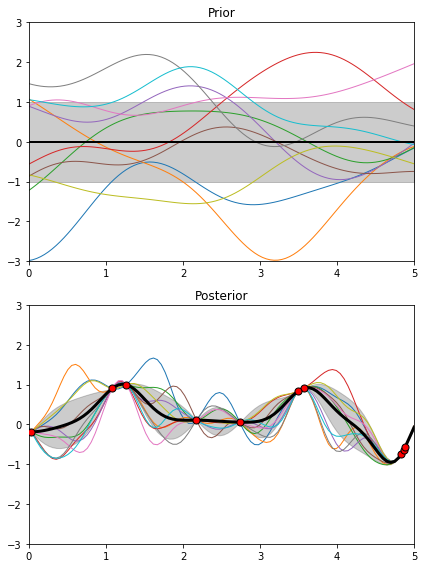
\includegraphics[width=0.6\linewidth]{gp.png}
		\caption{The upper panel is the $prior$ of a Gaussian Process with its parameters set at initial value. The bold black line is the mean, which in our example is constantly zero. The colored lines are sample functions drawn from this Gaussian Process. Grey area is one standard deviation away from the mean at each input point. The lower panel is the $posterior$. The dots on the black line are our observations. Colored lines are sample functions drawn from the $posterior$ distribution. Grey area is one standard deviation away from the mean. Notice that once we have our observation, we are more certain about the function value around observed points. This is illustrated by the shrinking of the grey area in the lower panel.}
		\label{fig:gp}
	\end{figure}
	
	Before one observes any values from a Gaussian Process, one only has a $prior$ distribution over functions specified by that Gaussian Process which may include all the continuous functions. Once some data points have been observed, the possible functions are now reduced to those that go through the observed points. Because of the multivariate gaussian distribution property of any finite subset of a Gaussian Process, one can compute the distribution of the points that one wants to predict conditioning on the observed points. $Prior$ combined with observation gives the $posterior$ distribution over the function that one wants to model.
	
	When there are more data points coming in, the uncertainty from the posterior distribution will be decreased. Hence, the prediction will become more and more confident when the model has observed more and more data. For traditional parametric methods, the model will tend to overfit the training data when the size of training set grows. However, for Gaussian Processes, since one are not assuming any specific form of the predicted function, one does not have to worry about overfitting of training data. There are still some flexibility left (specified by the variance of the posterior Gaussian distribution), even a lot of observation data points have been added to the prior distribution. 
	
	\subsection{Gaussian Process Regression}
	So far, we have introduced Gaussian Processes. In order to solve the regression problem, one needs to first define a $prior$ distribution of the target functions by a Gaussian process, then apply Bayesian inference to get the $posterior$ distribution of our predictions. The Gaussian Process Regression can be interpreted in two ways: 1) Weight-space View, and 2) Function-space View.
	
	\subsubsection{Weight-space View}
	The weight-space view of Gaussian Process starts with the standard linear regression model but from a Bayesian perspective. Recall the Bayesian linear regression model of input $\vec x$ and targets $y$ is
	\begin{equation}
	y = \vec x^T\vec w + \epsilon,
	\end{equation}
	where $\vec w$ is the weight and $\epsilon$ is Gaussian noise with distribution $\mathcal N(0,\sigma^2_n)$. This formulation gives the $likelihood$ of the training data
	\begin{equation}
	p(\vec y|\vec X, \vec w) = \mathcal N(\vec X^T\vec w,\sigma^2_nI).
	\end{equation}
	In the Bayesian setting, one needs to specify a $prior$ over the parameters $\vec w$ before we do any inference from the training data\cite[sec 2.1]{RandW}. We assume a zero mean Gaussian distribution for $\vec w$, $\vec w \sim \mathcal N(\vec 0, \Sigma)$. Then by Bayes' rule
	\begin{equation}
	posterior = \frac{likelihood \times prior}{\textit{marginal likelihood}},
	\end{equation}
	we have
	\begin{equation}
	p(\vec w|\vec y, \vec X) = \frac{p(\vec y|\vec X, \vec w)p(\vec w)}{p(\vec y | \vec X)},
	\end{equation}
	where \textit{marginal likelihood} is a constant and has the expression of
	\begin{equation}
	p(\vec y | \vec X) = \int p(\vec y|\vec X, \vec w) p(\vec w)d\vec w.
	\end{equation}
	Plug in $likelihood$ and $prior$ to get
	\begin{equation}
	p(\vec w|\vec y, \vec X) \propto \exp\left(-\frac{1}{2}(\vec w-\vec{\bar w})^T(\sigma^{-2}_n \vec X \vec X^T +\Sigma^T)(\vec w-\vec{\bar w})\right),
	\end{equation}
	where $\vec{\bar w}=\sigma^{-2}_n(\sigma^{-2}_n\vec X\vec X^T+\Sigma^{-1})^{-1}\vec X\vec y$. Notice that this is the probability density function of the $posterior$ of $\vec w$. We have the $posterior$ probability is
	\begin{equation}
	p(\vec w|\vec y, \vec X) = \mathcal N(\vec{\bar w},\bar \Sigma)
	\end{equation}
	where $\bar \Sigma = (\sigma^{-2}_n\vec X\vec X^T+\Sigma^{-1})^{-1}$.
	The prediction on a new data point $\vec x^*$ is the weighted average from all possible values of parameters by their $posterior$ distribution. Thus the predictive distribution for $y^*$ is 
	\begin{equation}\label{weight_space_pred}
	\begin{split}
	p(y^*|\vec x^*,\vec X, \vec y) &= \int p(y^*|x^*,\vec w)p(x|\vec W,\vec y)d\vec w\\
	&=\mathcal N\left(\sigma^{-2}_nx^{*T}\bar \Sigma \vec X\vec y,x^{*T}\bar\Sigma x^*\right).
	\end{split}
	\end{equation}
	
	The Bayesian linear model may perform poorly on higher dimensional data because of its  lack of complexity. One way to tackle this problem is to introduce a kernel function applying to the input data before doing linear regression. This approach will lead to the weight-space interpretation of Gaussian Process.
	
	Apply kernel function $\phi(\vec x)$ to the input, and the model becomes
	\begin{equation}
	y = \phi(\vec x)^T\vec w + \epsilon.
	\end{equation}
	Apply the same inference process as the standard Bayesian linear model above and replace $\vec X$ by $\Phi(\vec X)$, $\vec x^*$ by $\phi(\vec x^*)$in eq.\ref{weight_space_pred}, we get
	\begin{equation}
	p(y^*|\vec x^*,\vec X, \vec y) =\mathcal N\left(\sigma^{-2}_n\phi(x^*)^{T}\bar\Sigma\Phi \vec y,\phi(x^*)^{T}\bar\Sigma\phi(x^*)\right).
	\end{equation}
	Rewrite the above equation to get
	\begin{equation}\label{weight_space_pred_2}
	\begin{split}
	p(y^*|\vec x^*,\vec X, \vec y) =\mathcal N( &(\phi^*)^T\Sigma\Phi(K+\sigma^2_nI)^{-1}\vec y,\\
	&(\phi^*)^T\Sigma\phi^*- (\phi^*)^T\Sigma\Phi(K+\sigma^2_nI)^{-1}\Phi^T\Sigma \phi^*),
	\end{split}
	\end{equation}
	where $\phi^*=\phi(\vec x)^*$ and $K$ is defined as $\Phi^T\Sigma\Phi$.
	Notice that in eq.\ref{weight_space_pred_2}, one can interpret $(\phi^*)^T\Sigma\Phi$, $(\phi^*)^T\Sigma\phi^*$ and $\Phi^T\Sigma \phi^*$ as inner products with respect to $\Sigma$. If we define $\psi(\vec x) = \Sigma^{1/2}\phi(\vec x)$ and $k(\vec x,\vec x')=\psi(\vec x) \cdot \psi(\vec x') $, then we have $(\phi^*)^T\Sigma\Phi = k(\vec x^*,\vec X)$, $(\phi^*)^T\Sigma\phi^* = k(\vec x^*,\vec x^*)$ and $\Phi^T\Sigma \phi^* = k(\vec X,\vec x^*)$. Then eq. \ref{weight_space_pred_2} becomes
	\begin{equation}\label{weight_pred}
	\begin{split}
	p(y^*|\vec x^*,\vec X, \vec y) =\mathcal N(k&(\vec x^*,\vec X)(K+\sigma^2_nI)^{-1}\vec y,\\
	&k(\vec x^*,\vec x^*)- k(\vec x^*,\vec X)(K+\sigma^2_nI)^{-1}k(\vec X,\vec x^*)),
	\end{split}
	\end{equation}
	which is the predictive distribution of $y^*$ in Gaussian Process. 
	
	\subsubsection{Function-space View}
	Another interpretation of Gaussian Process Regression is through function-space view. If we consider a Gaussian Process as a continuous stochastic process, then it defines a probability distribution for functions \cite{Papoulis}. Since a multivariate Gaussian distribution can be completely specified by its mean and covariance, by definition \ref{def:gp}, then a Gaussian Process can be fully specified by its mean function and covariance function \cite{RandW}. If we define the mean function as $m(\vec{x})$ and covariance function $k(\vec{x},\vec{x'})$ of a real-valued Gaussian Process $f(\vec x)$ as
	\begin{equation} \label{}
	\begin{split}
	m(\vec{x}) & = \EE \left[ f(\vec x)\right] \\
	k(\vec{x},\vec{x'}) & = \EE \left[ \left( f(\vec x)-m(\vec{x})\right)\left( f(\vec x')-m(\vec{x'})\right)\right] 
	\end{split}
	\end{equation}
	
	and then one can write the Gaussian Process $f(\vec x)$ as
	\begin{equation} \label{}
	f(\vec x) \  \sim \ \GP\left(m(\vec{x}),k(\vec{x},\vec{x'})  \right).
	\end{equation}
	
	Suppose we choose a finite subset of random variables $\vec f$ from the Gaussian Process $f(\vec x)$, with the corresponding index set $\mathcal X$, then by definition of Gaussian Process, we know the distribution of $\vec f$:
	\begin{equation} \label{}
	p\left(\vec f \mid \mathcal X\right)\ =\ \mathcal N \left(\vec m , K \right),
	\end{equation}
	where $\mathcal N \left(\vec m , K \right)$ denotes a multivariate Gaussian distribution with mean $\vec m$ and covariance $K$. 
	In our task, the index set $\mathcal X$ can be a subset of $\mathbb R ^d$, where $d$ is the dimension of our input space. Usually we take the mean function to be a constant function equals to zero for notational simplicity. In practice, one can subtract the mean to achieve this. 
	
	If the target function $f(\vec x)$ is estimated as a Gaussian process, then one needs to check if the $consistency$ requirement of estimator is fulfilled. One can easily do this by the marginalization property of multivariate Gaussian distributions. The marginalization property tells us that if 
	\begin{equation*} \label{}
	\left(\vec f_1, \vec f_2\right)\ \sim \ \mathcal N \left(\vec m , K \right),
	\end{equation*}
	
	then we also have 
	\begin{equation*} \label{}
	\begin{split}
	\vec f_1\ & \sim \ \mathcal N \left(\vec m_1 , K_{11} \right)\\
	\vec f_2\ & \sim \ \mathcal N \left(\vec m_2 , K_{22} \right).
	\end{split}
	\end{equation*}
	where $K_{11}$ and  $K_{22}$ are sub-matrices of $K$. The proof is in the following:
	\begin{proof}
		We prove the marginal density $p(\vec f_1)$ follows Gaussian distribution. First, by definition of marginalization, we have
		\begin{equation*} \label{}
		p(\vec f_1) = \int p(\vec f_1,\vec f_2)d \vec f_2,
		\end{equation*}
		where 
		\begin{equation*} \label{}
		p(\vec f_1,\vec f_2) = \frac{1}{(2\pi)^{n/2}\sqrt{\det K}}\exp{(E)}
		\end{equation*}
		and $E$ is given by
		\begin{equation*} \label{}
		\begin{split}
		E &= -\frac{1}{2}\left(\vec f_2-(\vec m_2 - \vec\Lambda_{22}^{-1} \vec\Lambda_{21}(\vec f_1 - \vec m_1))\right)^T\vec\Lambda_{22}\left(\vec f_2-(\vec m_2 - \vec\Lambda_{22}^{-1} \vec\Lambda_{21}(\vec f_1 - \vec m_1))\right)\\
		&+\frac{1}{2}\left(\vec f_1^T \vec\Lambda_{12}\Lambda_{22}^{-1}\Lambda_{21}\vec f_1 - 2\vec f_1^T \vec\Lambda_{12}\Lambda_{22}^{-1}\Lambda_{21}\vec m_1 + \vec m_1^T \vec\Lambda_{12}\Lambda_{22}^{-1}\Lambda_{21}\vec m_1\right)\\
		&-\frac{1}{2}\left(\vec f_1^T\Lambda_{11}\vec f_1 - 2\vec f_1^T\Lambda_{11}\vec m_1 + \vec m_1^T\Lambda_{11}\vec m_1\right)\\
		&=-\frac{1}{2}\left(\vec f_2-(\vec m_2 - \vec\Lambda_{22}^{-1} \vec\Lambda_{21}(\vec f_1 - \vec m_1))\right)^T\vec\Lambda_{22}\left(\vec f_2-(\vec m_2 - \vec\Lambda_{22}^{-1} \vec\Lambda_{21}(\vec f_1 - \vec m_1))\right)\\
		&-\frac{1}{2}\left(\vec f_1 - \vec m_1\right)^T\left(\vec\Lambda_{11}-\vec\Lambda_{12}\vec\Lambda_{22}^{-1}\vec\Lambda_{21}\right)\left(\vec f_1 - \vec m _1 \right)
		\end{split}
		\end{equation*}
		where $\vec\Lambda$ is the information matrix and
		\begin{equation*} \label{}
		\vec \Lambda = K^{-1} = 
		\begin{pmatrix}
		\vec\Lambda_{11} & \vec\Lambda_{12}\\
		\vec\Lambda_{21} & \vec\Lambda_{22}
		\end{pmatrix}.
		\end{equation*}
		Using the \textit{matrix inversion lemma} (see Appendix), we have
		\begin{equation*} \label{}
		K_{11}^{-1} = \vec\Lambda_{11}-\vec\Lambda_{12}\vec\Lambda_{22}^{-1}\vec\Lambda_{21},
		\end{equation*}
		combined with the line above to get
		\begin{equation*} \label{}
		p(\vec f_1,\vec f_2) = \frac{1}{(2\pi)^{n/2}\sqrt{\det K}}\exp{(E_1)}\exp{(E_2)},
		\end{equation*}
		where
		\begin{equation*} \label{}
		\begin{split}
		E_1 &=-\frac{1}{2}\left(\vec f_2-(\vec m_2 - \vec\Lambda_{22}^{-1} \vec\Lambda_{21}(\vec f_1 - \vec m_1))\right)^T\vec\Lambda_{22}\left(\vec f_2-(\vec m_2 - \vec\Lambda_{22}^{-1} \vec\Lambda_{21}(\vec f_1 - \vec m_1))\right)\\
		E_2 & = -\frac{1}{2}\left(\vec f_1 - \vec m_1\right)^T\left(\vec\Lambda_{11}-\vec\Lambda_{12}\vec\Lambda_{22}^{-1}\vec\Lambda_{21}\right)\left(\vec f_1 - \vec m _1 \right).
		\end{split}
		\end{equation*}
		Since $E_2$ is independent of $\vec f_1$, we have
		\begin{equation*} \label{}
		p(\vec f_1) = \frac{1}{(2\pi)^{n/2}\sqrt{\det K}}\int \exp{(E_1)}d\vec f_2\exp{(E_2)}.
		\end{equation*}
		Integral of a probability density function is one, we get
		\begin{equation*} \label{}
		\int \exp{(E_1)}d\vec f_2 = (2\pi)^{n_2/2}\sqrt{\det \vec \Lambda_{22}^{-1}}
		\end{equation*}
		plug this into the line above to get
		\begin{equation*} \label{}
		p(\vec f_1) = \frac{\sqrt{\det \vec \Lambda_{22}^{-1}}}{(2\pi)^{n_1/2}\sqrt{\det K}} \exp{\left(-\frac{1}{2}\left(\vec f_1 - \vec m_1\right)^TK_{11}^{-1}\left(\vec f_1 - \vec m _1 \right)\right)}.
		\end{equation*}
		Again, by the \textit{matrix inversion lemma}, we have
		\begin{equation*} \label{}
		\begin{split}
		\det K&= \det K_{11}\det(K_{22}-K_{21}K_{11}^{-1}K_{12})\\
		\vec \Lambda_{22}^{-1} &= K_{22}-K_{21}K_{11}^{-1}K_{12}.
		\end{split}
		\end{equation*}
		Plug those results into the previous line, we get
		\begin{equation*} \label{}
		p(\vec f_1) = \frac{1}{(2\pi)^{n_1/2}\sqrt{\det K_{11}}} \exp{\left(-\frac{1}{2}\left(\vec f_1 - \vec m_1\right)^TK_{11}^{-1}\left(\vec f_1 - \vec m _1 \right)\right)}.
		\end{equation*}
		which proves that $\vec f_1\sim\mathcal{N}(\vec m_1,K_{11})$.
	\end{proof}
	
	Through $consistency$ of Gaussian process, one knows if $\left(\vec f_1, \vec f_2\right)\sim \mathcal N \left(\vec m , K \right)$, then $\vec f_1 \sim   \mathcal N \left(\vec m_1 , K_{11} \right)$ and $ \vec f_2 \sim  \mathcal N \left(\vec m_2 , K_{22} \right)$. Now one can use Gaussian process to model target function that one wants to estimate.
	
	Firstly, model the target latent function $\vec f$ by a zero mean Gaussian Process, then $\vec f$ has prior distribution:
	\begin{equation} \label{noise-free}
	\vec f \sim \mathcal{N}(\vec 0, K),
	\end{equation}
	where $K$ is the covariance matrix.
	
Assume the special case where the target functions are noise-free. Suppose we have observed data $\{(\vec x_i,f_i)|i=1,...,n\}$, we want to infer the value of our target function at input points $\{\vec x_j | j = 1,...,n_*\}$. We call $\vec f$ as training outputs and $\vec f_*$ as test outputs. From the prior distribution, we know 
	$\vec f$ and $\vec f_*$ have joint distribution
	\begin{equation} \label{}
	\begin{bmatrix}
	\vec f\\
	\vec f_*
	\end{bmatrix}
	\sim
	\mathcal{N}\left(\vec 0, 
	\begin{bmatrix}
	K(\vec X,\vec X) & K(\vec X,\vec X_*)\\
	K(\vec X_*,\vec X) & K(\vec X_*,\vec X_*)
	\end{bmatrix}
	\right).
	\end{equation}
	$K(\vec X,\vec X)$ denotes the covariance matrix of $n$ training data points, $K(\vec X_*,\vec X_*)$ denotes the covariance of $n_*$ test data points and $K(\vec X_*,\vec X)$ denotes the cross-covariance of training and test data points. To get the distribution of our prediction on the test data set, we just condition the joint Gaussian prior distribution on the training data set. Then we get
	\begin{equation} \label{eq:pred1}
	\vec f_* | \vec X_*, \vec X, \vec f \sim \mathcal N (\vec m_*, V_*),
	\end{equation}
	where
	\begin{equation} \label{eq:pred2}
	\begin{split}
	\vec m_* &= K(\vec X_*,\vec X)K(\vec X,\vec X)^{-1}\vec f,\\
	V_* &= K(\vec X_*,\vec X_*) - K(\vec X_*,\vec X)K(\vec X,\vec X)^{-1}K(\vec X,\vec X_*).
	\end{split}
	\end{equation}
	
	\begin{proof}
		For notational simplicity, let's denote $K(\vec X,\vec X)$ as $K$, $K(\vec X,\vec X_*)$ and $K(\vec X_*,\vec X)$ as $K_*$ and $K(\vec X_*,\vec X_*)$ as $K_{**}$.
		
		The conditional probability density function of $\vec f_*$ given $\vec f$ is 
		\begin{equation}\label{conditional_pdf}
		p(\vec f_*|\vec f) = \frac{p(\vec f, \vec f_*)}{\int p(\vec f,\vec f_*)d\vec f},
		\end{equation}
		where $\int p(\vec f,\vec f_*)d\vec f$ is a normalization constant. Denote the normalization constant as $E$, we have
		\begin{equation}
		p(\vec f_*|\vec f) = \frac{1}{E}\exp \left(-\frac{1}{2}
		\begin{bmatrix}
		\vec f\\
		\vec f_*
		\end{bmatrix}^T
		\begin{bmatrix}
		K & K_*\\
		K_* & K_{**}
		\end{bmatrix}^{-1}
		\begin{bmatrix}
		\vec f\\
		\vec f_*
		\end{bmatrix}
		\right).
		\end{equation}
		Denote 
		\begin{equation}
		\begin{bmatrix}
		K & K_*\\
		K_* & K_{**}
		\end{bmatrix}^{-1}
		=
		\begin{bmatrix}
		V & V_*\\
		V_* & V_{**}
		\end{bmatrix},
		\end{equation}
		then we get
		\begin{equation}
		\begin{split}
		p(\vec f_*|\vec f) &= \frac{1}{E}\exp \left(-\frac{1}{2}
		\begin{bmatrix}
		\vec f\\
		\vec f_*
		\end{bmatrix}^T
		\begin{bmatrix}
		V & V_*\\
		V_* & V_{**}
		\end{bmatrix}
		\begin{bmatrix}
		\vec f\\
		\vec f_*
		\end{bmatrix}
		\right)\\
		&=\frac{1}{E}\exp\left(-\frac{1}{2}[\vec f^T V \vec f+\vec f^T V_* \vec f_* +\vec f_*^T V_* \vec f +\vec f_*^T V_{**}\vec f_*]\right).
		\end{split}
		\end{equation}
		Complete the square to get
		\begin{equation}
		\begin{split}
		p(\vec f_*|\vec f) = \frac{1}{E}\exp(-[&\frac{1}{2}(\vec f_* +V^{-1}_{**}V_* \vec f)^T V_{**}(\vec f_* + V^{-1}_{**}V_* \vec f)\\
		&\frac{1}{2}\vec f^T V \vec f - \frac{1}{2}\vec f^T V_* V^{-1}_{**}V_*\vec f]).
		\end{split}
		\end{equation}
		Take out the terms that are independent of $\vec f_*$ from the exponential and put them into the normalization constant to get updated constant $E'$, then we get
		\begin{equation}
		p(\vec f_*|\vec f) = \frac{1}{E'}\exp\left(-\frac{1}{2}(\vec f_* +V^{-1}_{**}V_*\vec f)^TV_{**}(\vec f_* ++V^{-1}_{**}V_*\vec f)\right).
		\end{equation}
		Recognise this is in the form of Gaussian probability density function with 
		\begin{equation}
		\begin{split}
		\vec \mu &= -V^{-1}_{**}V_*\vec f,\\
		\sigma^2 &= V_{**}^{-1}.
		\end{split}
		\end{equation}
		By \textit{matrix inverse lemma}(see Appendix), we have
		\begin{equation}
		\begin{bmatrix}
		K & K_*\\
		K_* & K_{**}
		\end{bmatrix}
		=
		\begin{bmatrix}
		(V-V_*V^{-1}_{**}V_*)^{-1} & -(V-V_*V^{-1}_{**}V_*)^{-1}V_*V^{-1}_{**}\\
		-V^{-1}_{**}V_*(V-V_*V^{-1}_{**}V_*)^{-1} & (V_{**}-V_*V^{-1}V_*)^{-1}
		\end{bmatrix}.
		\end{equation}
		Combining the previous line to get
		\begin{equation}
		\begin{split}
		\vec \mu &= -V^{-1}_{**}V_*\vec f = K_*K^{-1}\vec f,\\
		\sigma^2 &= V_{**}^{-1} = K_{**}-K_*K^{-1}K_*,
		\end{split}
		\end{equation}
		which concludes the proof for eq.\ref{eq:pred1} and \ref{eq:pred2}.
	\end{proof}
	
	Our prediction of the test set is a $posterior$ Gaussian distribution with mean $\vec m_*$ and covariance $\vec V_*$.  Notice that in our prediction, rather than giving specific parametric relationship between the test input $\vec X_*$ and the prediction value, we just give a Gaussian distribution inferred from our prior distribution and observation. If we want to get an exact value of $\vec f_*$ for prediction, we can sample from the posterior distribution or simply take the mean $\vec m_*$ as our prediction. For more on this, see section \ref{sec:decision_theory}. We can also get the variance $v_*$ of each individual element in vector  $\vec f_*$ from the covariance matrix $\vec V_*$. The smaller the variance is, the more confident we are about the prediction. 
	
	In most real-life application, it is more realistic to incorporate noise in our target values. We can denote the noisy target values as $\vec y$ in training set. We then write the noisy value as $\vec y = f(\vec x) + \vec\epsilon$. Assuming identical, independent Gaussian noise $\vec \epsilon$ with mean $0$ and variance $\sigma^2_n$, then the covariance on the noisy observation is
	\begin{equation*} \label{}
	\mathrm{cov} (y_i,y_j) = k(\vec x_i,\vec x_j) + \sigma^2_n \delta_{ij}
	\end{equation*}
	where $\delta_{ij}$ is a Kronecker delta which is $1$ is $i=j$ and $0$ otherwise. The above relationship is vector form is
	\begin{equation} \label{cov_y}
	\mathrm{cov} (\vec y) = K(X,X) + \sigma^2_n \vec I,
	\end{equation}
	where the identity matrix $\vec I$ comes from the independence assumption of the noise. Then we can write the joint prior distribution of noisy training data and test data as
	\begin{equation} \label{}
	\begin{bmatrix}
	\vec y\\
	\vec f_*
	\end{bmatrix}
	\sim
	\mathcal{N}\left(\vec 0, 
	\begin{bmatrix}
	K(X,X)+ \sigma^2_n \vec I & K(X,X_*)\\
	K(X_*,X) & K(X_*,X_*)
	\end{bmatrix}
	\right).
	\end{equation}
	Then by the same derivation to eq. \ref{eq:pred1} and \ref{eq:pred2}, we get the prediction for test data. The posterior distribution is 
	\begin{equation} \label{eq:pred3}
	\vec f_* | X_*, X, \vec y \sim \mathcal N (\widehat{\vec m_*}, \widehat{\vec V_*}),
	\end{equation}
	where
	\begin{equation} \label{eq:pred4}
	\begin{split}
	\widehat{\vec m_* }&= K(X_*,X)[K(X,X)+ \sigma^2_n \vec I]^{-1}\vec y,\\
	\widehat{\vec V_*} &= K(X_*,X_*) - K(X_*,X)[K(X,X)+ \sigma^2_n \vec I]^{-1}K(X,X_*).
	\end{split}
	\end{equation}
This is equivalent to the predictive distribution from weight-space view in eq.\ref{weight_pred}.
	
	Notice that though we assume the mean function as constantly zero in the prior distribution, we get non-zero mean function in the posterior distribution for the test data set. This can be interpreted as after observing the training set, the model has more information about the distribution of the test set. Also, different from a parametric model, the Gaussian Process Regression model needs to store all the training data for prediction. For a parametric model, the goal is to find the predefined parametric relationship between features and targets, once done that, the model doesn't need the training data for prediction. The features, ${\vec x^*_i | i=1,...,n^*}$, will give all the information we need for prediction $\vec y^*_i$'s. However, in Gaussian Process Regression model, the prediction eq. \ref{eq:pred3} and eq. \ref{eq:pred4} need the information from training set to get the posterior distribution of the test set.
	
	\subsection{Predicition from Gaussian Process Regression}\label{sec:decision_theory}
	Form eq. \ref{eq:pred3}, we know that the posterior distribution of test data is Gaussian with mean and variance given in eq.\ref{eq:pred4}. But if one wants an explicit prediction for the target function rather than a distribution, what is the value then? One intuitive answer would be the mean of posterior distribution. In practice, this prediction is appropriate in most real-life tasks. Rasmussen and Williams provides in-depth explanation in \cite[sec 2.4]{RandW}, we present a summary of the rationale in the following.
	
	To find a optimal prediction value, we need a way to measure our performance. Let's define a \textit{loss function}, $\mathcal{L}(\hat y,y)$, which specifies the loss between the prediction, $\hat y$ and the true value, $y$. The loss function can be \textit{mean squared error} or \textit{mean absolute error} which are both symmetric loss functions.
	
	We want to give a prediction value that produces the minimum loss possible. But how do we achieve that when we don't know the true value? According to \cite[Rasmussen and Williams, sec 2.4]{RandW}, we can minimize the expected loss, by averaging the loss with respect to the posterior distribution, which is 
	\begin{equation}\label{loss1}
	\tilde{R}_{\mathcal{L}}(\hat y|\vec x_*)\ = \ \int\mathcal{L}(y_*,\hat y)p(y_*|\vec x_*)dy_*.
	\end{equation}\label{loss2}
	Our best prediction is the one that minimizes this loss, i.e.
	\begin{equation}
	y_{optimal}|\vec x_*\ = \ \underset{\hat y}{\mathrm{argmin}}\tilde{R}_{\mathcal{L}}(\hat y|\vec x_*).
	\end{equation}
	For \textit{mean squared error} loss function, the minimum occurs at the mean of $y_*$. For \textit{mean absolute error} loss function, the minimum occurs at the median of $y_*$. In our case, the distribution of $y_*$ is Gaussian, so the mean and median coincide. Furthermore, for other symmetric loss function and symmetric posterior distribution, the optimal prediction occurs at the mean of the distribution. For asymmetric loss functions, the optimal prediction can be computed from eq. \ref{loss1} and eq. \ref{loss2}. For more detail, see \cite{Berger}.
	
	\newpage
	\section{Model Selection}\label{sec:model_selection}
	When modelling the target function as a zero mean Gaussian process, i.e.
	\begin{equation*} \label{}
	f(\vec x) \  \sim \ \GP\left(\vec 0,k(\vec{x},\vec{x'})  \right).
	\end{equation*}
	the main task will be to find a good configuration of covariance matrix, generated by kernel function $k$ and a set of $hyperparameters$ that gives the best performance. The model selection is a combination of choosing a good kernel function and optimizing $hyperparameters$ of the kernel function. In this section, we will discuss several aspects of model selection, namely marginal likelihood, covariance matrix, kernel functions, $hyperparameters$ optimization.
	
	\subsection{Marginal Likelihood of the training data}\label{lik}
	From eq. \ref{noise-free}, the noise-free $prior$ follows multivariate Gaussian distribution with mean $\vec 0$ and covariance matrix $K(X,X)$. By Bayes' theorrm, the marginal likelihood of the noisy training data is the integral of the likelihood times prior, which is 
	
	\begin{equation}
	p(\vec y|X)\, = \, \int p(\vec y|\vec f, X)p(\vec f|X)d\vec f.
	\end{equation}
	
	The term \textit{marginal} likelihood means the marginalization over the function values $\vec f$. Assume identical, independent Gaussian noise, then we have $\vec y = f(\vec x) + \vec\epsilon$, where $\vec\epsilon \sim \mathcal{N}(\vec 0, \sigma^2_n)$. Let $K_y = K + \sigma^2_nI$, then by eq. \ref{cov_y}. one gets
	\begin{equation}
	\vec y \  \sim \ \mathcal N \left(\vec 0,K_y  \right).
	\end{equation}
	Since the likelihood of a Gaussian distribution involves exponential term, one can take the logarithm of it. The log likelihood of $\vec y$ given $\vec X$ and $\vec \theta$ is 
	\begin{equation}\label{log-likelihood}
	\log p(\vec y|\vec X, \vec \theta)=-\frac{1}{2}\vec y^T K_y^{-1}\vec y-\frac{1}{2}\log|K_y| - \frac{n}{2}\log 2\pi,
	\end{equation}
	where $\vec \theta$ is parameters in kernel function $k$.
	
	\subsection{Covariance Matrix and Kernel functions}\label{subsec:kernel_func}
	A kernel function $k$ (also called a covariance function) governs the behaviour and property of a zero-mean Gaussian process. Since for any element $K_{ij}$ in the covariance matrix $K$, we know $K_{ij} = k(\vec x_i,\vec x_j)$, the relationship of covariance matrix $K$ and kernel function $k$ is
	\begin{equation}\label{cov_mat}
	K = 
	\begin{bmatrix}
	k(\vec x_1,\vec x_1) & k(\vec x_1,\vec x_2)& \dots& k(\vec x_1,\vec x_n)\\
	k(\vec x_2,\vec x_1) & k(\vec x_2,\vec x_2)& \dots& k(\vec x_2,\vec x_n)\\
	\vdots & \vdots  & \ddots & \vdots \\
	k(\vec x_n,\vec x_1) & k(\vec x_n,\vec x_2)& \dots& k(\vec x_n,\vec x_n)
	\end{bmatrix}
	\end{equation}
	
	%ADD GRAPH TO ILLUSTRATE COVARIANCE MATRIX
	
	\begin{figure}[h!]
		\centering
		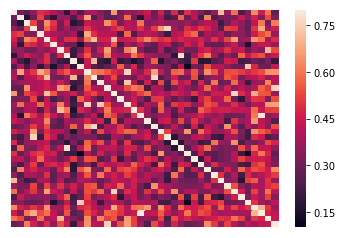
\includegraphics[width=0.49\textwidth]{cov1.png}
		\hspace{0.15em}
		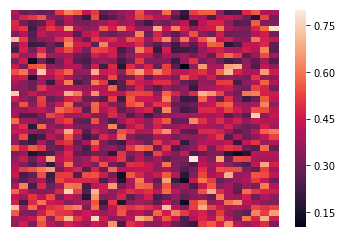
\includegraphics[width=0.49\textwidth]{cov2.png}
		\caption{Heat-map of Covariance matrices. The left panel is the covarianve matrix $K$ of the training data $\vec X$. The diagonal component $K_{ii}$ is the variance of $\vec X_i$, the off-diagonal component $K_{ij}$ is the covariance between $\vec X_i$ and $\vec X_j$. The right panel is the cross-covariance $K^*$ of $\vec X$ and testing data $\vec X^*$. $K^*_{ij}$ is the covariance between $\vec X_i$ and $\vec X^*_j$.}
	\end{figure}
	
	A kernel function in some sense measures the similarity between two data points in the input space. The basic assumption in GPR is that two points that are close in the input space should be more likely to have similar target values. 
	
	Since a covariance matrix is always positive-semidefinite\footnotemark[1] and symmetric, for a function to be qualified as a kernel function, it must be positive-semidefinite\footnotemark[2] and symmetric in the sense that $k(\vec x_i,\vec x_j) = k(\vec x_j,\vec x_i)$\cite[sec 4.1]{RandW}.
	
	\footnotetext[1]{
		A symmetric $n\times n$ real matrix $\vec M$ is said to be positive-semidefinite(PSD) if $\vec v^T\vec M\vec v$ is non-negative for all $\vec v$ in $\RR^n$.
	}
	\footnotetext[2]{
		A $kernel$ is said to be positive-semidefinite if 
		\[
		\int k(\vec x,\vec x')f(\vec x)f(\vec x')d\mu(\vec x)d\mu(\vec x')\, \geq 0,
		\]
		for all $f\in L_2(\mathcal X,\mu)$, $\mathcal X$ is the input space and $\mu$ is a measure.
	}
	
	\subsubsection{Several Common Kernel functions}
	To understand what kind of function structure that Gaussian process can express, one has to first understand properties of embedded kernel function of the GP.
	Kernel function map $\vec x,\vec x' \in \mathcal X$ into $\RR$. The similarity of $\vec x,\vec x'$ in $\mathcal X$ is measured by the result from the kernel function.
	
	A stationary kernel function is a function whose value only depends on the difference between $\vec x$ and $\vec x'$. One can write $k$ to take only single argument $\vec r = \vec x - \vec x'$. 
	\subsubsection*{Radial Basis Function Kernel}
	The mostly commonly used stationary kernel function is the \textit{Radial Basis Function}(RBF) kernel, which has the form
	\begin{equation}\label{RBF}
	k_{RBF}\, = \, \sigma^2\exp\left(-\frac{\vec r^2}{2l^2}\right),
	\end{equation}
	where the parameter $l$ is the \textit{characteristic length-scale} and $\sigma$ controls the magnitude of function value. The RBF kernel function is also known as the \textit{quared exponential}(SE) function. This kernel function has derivatives at all orders, which means Gaussian process with this kernel will be very smooth. For detailed explanation, please see \cite[sec 4.2]{RandW}. Sometimes, target functions in real wrold application do not have this smoothness, so another family of stationary kernel functions, namely the \textit{Mat\'ern class} kernel functions are introduced by Stein in \cite{Stein}.
	
	\subsubsection*{Mat\'ern Class of Kernel Functions}
	This class of kernel functions was named after the work of Mat\'ern. The general form of \textit{Matern class} kernel functions is given by
	\begin{equation}
	k_{Matern}(\vec r) = \frac{2^{1-\nu}}{\Gamma{(\nu)}}\left(\frac{\sqrt{2\nu}\vec r}{l}\right)^\nu K_\nu \left(\frac{\sqrt{2\nu}\vec r}{l}\right),
	\end{equation}
	where $\nu$ and $l$ are positive parameters and $K_\nu$ is a second kind modified Bessel function\cite[sec 9.6]{Ab_St}. When $\nu \rightarrow \infty$, we obtain the SE kernel function. For smaller $\nu$, the resulting Gaussian process has a rougher path than those from a SE kernel. The most commonly exploited cases in machine learning is when $\nu = 3/2$ and $ 5/2$ \cite[sec 4.2]{RandW}. These two kernel functions are of the forms
	\begin{equation}
	\begin{split}
	k_{Matern32}(\vec r) &=\left(1+\frac{\sqrt{3}\vec r}{l}\right)\exp\left(-\frac{\sqrt{3}\vec r}{l}\right),\\
	k_{Matern52}(\vec r) &=\left(1+\frac{\sqrt{5}\vec r}{l}+\frac{5\vec r^2}{3l^2}\right)\exp\left(-\frac{\sqrt{5}\vec r}{l}\right).
	\end{split}
	\end{equation}
	For $\nu\geq 7/2$, Rasmussen and Williams have proved the resulting Gaussian process is very smooth in \cite[sec 4.2]{RandW}.
	
	Stationary kernels will give the same value as long as the difference between $\vec x$ and $\vec x'$ is the same. Hence, stationary kernels are translation invariant. When one wants to incorporate effects of translation in feature space, non-stationary kernel functions should be introduced.
	
	\begin{figure}[t!]
		\centering
		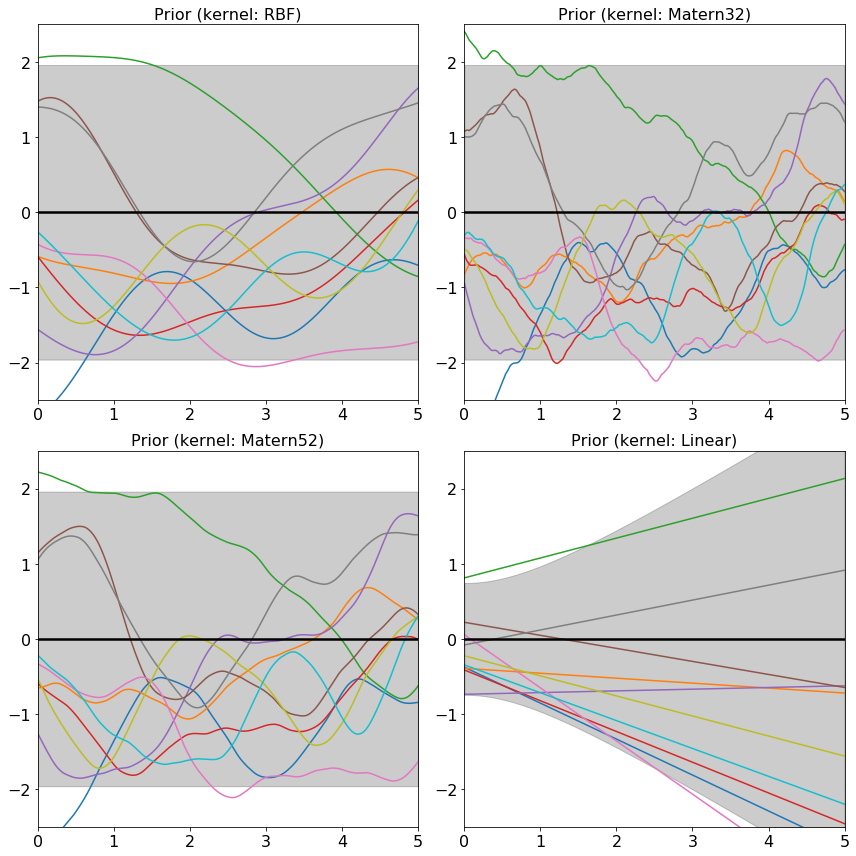
\includegraphics[width=.9\linewidth]{prior_diff_kernels.png}
		\caption{GP Priors with different kernels. For staiontionary kernels e.g. RBF, Matern32 and Matern53, variance at each point(covariance with itself) is constant for fixed parameters. For non-stationary kernel, e.g. Linear kernel, variance increases as data points move away from the origin. We can also see that sample functions drawn from $prior$ distribution of different kernels show different level of smoothness. Sample functions draw from Linear kernel are linear functions.}
		\label{fig:gp_diff_kernels}
	\end{figure}
	
	\subsubsection*{Linear Kernel Functions}
	A linear kernel function has the form
	\begin{equation}
	k_{Linear} = \frac{\vec x \cdot \vec x'}{l},
	\end{equation}
	where $l$ is the \textit{characteristic length-scale}. Gaussian process governed by a Linear kernel will estimate a linear function, see figure \ref{fig:gp_diff_kernels}. The expressive ability of Linear kernel alone is not very interesting, but combined with other non-linear kernel. the resulting GP can capture global trend as well as local variation of the target function. 
	
	GP $priors$ and $posteriors$ with different kernel functions are shown in Figure \ref{fig:gp_diff_kernels} and \ref{fig:gp_diff_kernels_2}.
	
	\begin{figure}[h!]
		\centering
		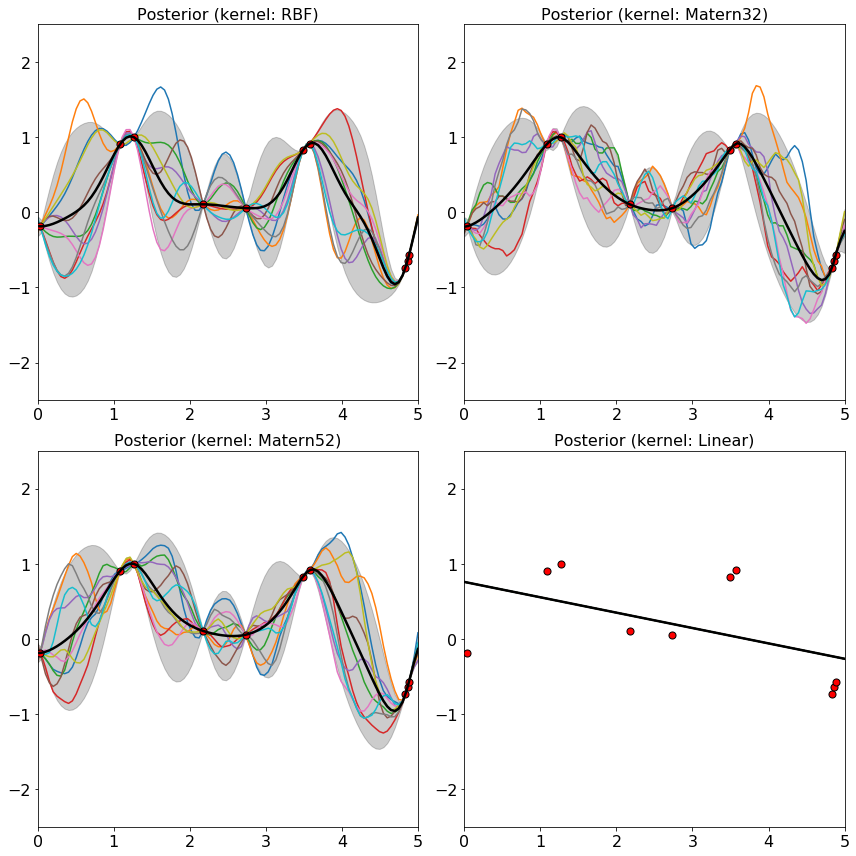
\includegraphics[width=.9\linewidth]{posterior_diff_kernels.png}
		\caption{GP Posteriors with different kernels. The red dots are the training points. The black line is the mean function, the grey area is 95\% confidence intervel.}
		\label{fig:gp_diff_kernels_2}
	\end{figure}
	
	\subsubsection*{Combining Kernel Functions}
	For most real-life tasks e.g. estimating the price of derivatives, using vanilla kernel functions described above may not generate ideal result. We can construct new kernel functions from these vanilla kernel functions by addition, multiplication, convolution and other methods. Adding two kernel functions is equivalently modelling the resulting Gaussian process by the sum of two independent Gaussian processes\cite[sec 4.2]{RandW}.
	
	\begin{figure}[h!]
		\centering
		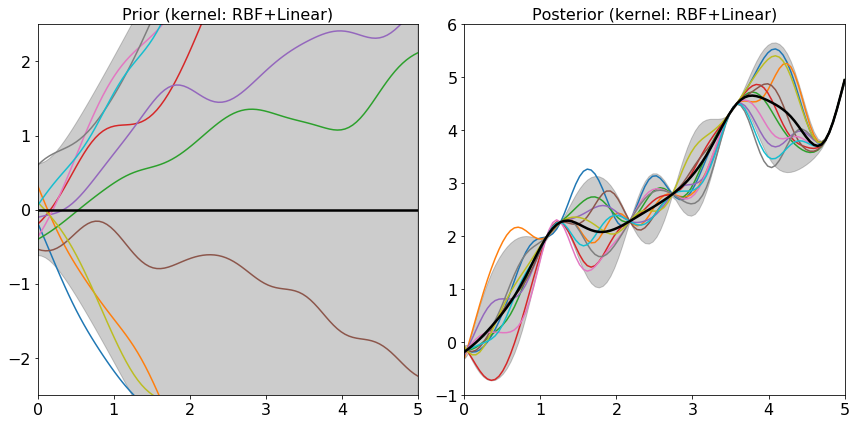
\includegraphics[width=.9\linewidth]{kernel_combo.png}
		\caption{GP $prior$ and $posterior$ with RBF+Linear kernel. The mean function from the $postetior$ distribution has a upwards trend and local variation.}
		\label{fig:gp_kernel_combo}
	\end{figure}
	
	\subsubsection{Optimizing Kernel Parameters}
	Each kernel function has a set of parameters which determines properties of the kernel function. In Gaussian process regression, since these parameters specify distributions of the parameters of target function, so we call them $hyperparameters$ of the model. In the training process of our model, we want to find a optimal set of $hyperparameters$ in the sense that the log likelihood of our training data define in eq. \ref{log-likelihood} is maximised. We will discuss in detail about training methods in the following subsection.
	
	\subsubsection{Numerical Results of Different Kernels}
	
	\begin{table}[h!]
		\centering
		\begin{tabular}{l|llll|llll} 
			\toprule
			& \multicolumn{4}{l|}{Training data absolute difference~ ~}          & \multicolumn{4}{l}{Testing data absolute difference~ ~}            \\
			& 10             & 100            & 1000           & 10000           & 10             & 100            & 1000           & 10000           \\ 
			\hline\hline
			RBF             & 59.31          & 78.02          & 95.31          & 99.28           & 27.66          & 36.97          & 50.50          & 75.85           \\
			Matern32        & \textbf{60.77} & 78.89          & 94.43          & 99.46           & \textbf{30.76} & 40.58          & \textbf{58.02} & \textbf{80.66}  \\
			Matern52        & 59.85          & 78.65          & 95.00          & 99.38           & 30.26          & 38.78          & 53.31          & 77.56           \\
			RBF+Linear      & 50.42          & 79.90          & \textbf{97.91} & \textbf{100.00} & 28.36          & 39.78          & 53.81          & 75.55           \\
			Matern32+Linear & 48.88          & 77.16          & 96.48          & 99.96           & 27.15          & 39.68          & 53.51          & 75.45           \\
			Matern52+Linear & 54.24          & \textbf{80.21} & 96.72          & 99.77           & 29.36          & \textbf{41.28} & 54.61          & 77.15           \\
			\bottomrule
		\end{tabular}
		\caption{Results for kernels with single value length-scale. }
		\label{table:res_single_lengthscale}
	\end{table}
	
	Table \ref{table:res_single_lengthscale} shows prediction performance of GPRs governed by different kernel functions namely RBF, Matern32, Matern52, RBF+Linear, Matern32+Linear and Matern52+Linear. The target function is the price of synthetic CDO. We divide the training set into 4 batches of 2048 points in each batch for computational efficiency. The testing set size is 998. The feature space $\mathcal X$ is $[0,1]^{1118}$. We measure the absolute value of difference between prediction and target value from 10 to 10000. The results are shown as the percentage of the entire testing set. GPR with Mat\'ern32 kernel function has the most prediction within absolute difference of 10 out of all other kernel functions. This can be explained by the smoothness by the target function that we are trying to estimate. Functions modelled GPR with Mat\'ern32 kernel are rougher than those by GPR with RBF and Mat\'ern52 function. When added Liner kernel function, the results do improve a little within absolute difference of 1000 and 10000 on training set, this means our model can explain more of the global trend of the target function compared to the one without Linear kernel. However, the performance get worse within the absolute difference of 10. This is maybe because the target function does not have a clear linear relationship with any of the dimensions from feature space, when fitted by a Linear kernel, the model is not able to give an accurate prediction.
	
	\subsubsection{Automatic Relevance Determination}
	In the previous discussion, we used single scalar value for the \textit{characteristic length-scale} $l$ in hyperparameter $\vec \theta$ for kernels functions. In practice, for multi-dimensional feature space, a universal \textit{characteristic length-scale} for all dimensions may not perform well. Instead, We can assign a \textit{characteristic length-scale} for each dimension. For instance, a RBF and Mat\'ern kernel function in this form are
	\begin{equation}\label{RBF_ARD}
	\begin{split}
	k_{RBF\_ARD}(\vec r)\, &= \, \sigma^2\exp\left(-\frac{1}{2}\sum_{i=1}^{d}\frac{\vec r^2_i}{ l^2_i}\right),\\
	k_{Matern32\_ARD}(\vec r) &=\left(1+\sqrt{3}\sum_{i=1}^{d}\frac{\vec |r_i|}{l_i}\right)\exp\left(-\sqrt{3}\sum_{i=1}^{d}\frac{\vec |r_i|}{l_i}\right),\\
	k_{Matern52\_ARD}(\vec r) &=\left(1+\sqrt{5}\sum_{i=1}^{d}\frac{\vec |r_i|}{l_i}+\frac{5}{3}\sum_{i=1}^{d}\frac{\vec r^2_i}{ l^2_i}\right)\exp\left(-\sqrt{5}\sum_{i=1}^{d}\frac{\vec |r_i|}{l_i}\right).
	\end{split}
	\end{equation}
	where $\vec r \in \mathbb R^d$, $d$ is the number of dimensions in feature space. ARD stands for automatic relevance determination\cite[Neal]{Neal}. 
	From eq.\ref{RBF_ARD}, we can see that the inverse of $l_i$ will determine how sensitive the covariance is to the change in $\vec r_i$. For large value of $l_i$, the inverse is close to zero which will make the value of covariance all-most invariant to the change in $\vec r_i$. This effect will determine the relevance of $i^{th}$ dimension of input to the covariance given enough training data, hence, the name -- automatic relevance determination.
	
	\begin{table}[h!]
		\centering
		\begin{tabular}{l|llll|llll} 
			\toprule
			& \multicolumn{4}{l|}{Training data absolute difference}             & \multicolumn{4}{l}{Testing data absolute difference}               \\
			& 10             & 100            & 1000           & 10000           & 10             & 100            & 1000           & 10000           \\ 
			\hline\hline
			RBF             & 47.94          & 74.13          & 94.06          & 99.96           & 27.45          & 41.58          & 65.83          & 88.38           \\
			Matern32        & \textbf{58.51} & \textbf{83.42} & \textbf{98.35} & 99.98           & \textbf{30.76} & 44.59          & 68.34          & 88.08           \\
			Matern52        & 56.10          & 81.23          & 97.52          & 99.98           & 29.56          & \textbf{45.29} & 68.44          & 87.88           \\
			RBF+Linear      & 31.30          & 56.18          & 85.61          & 99.63           & 23.75          & 39.48          & 65.23          & 89.78           \\
			Matern32+Linear & 45.19          & 75.07          & 96.25          & \textbf{100.00} & 28.36          & 41.98          & \textbf{68.74} & \textbf{90.28}  \\
			Matern52+Linear & 50.92          & 80.51          & 97.86          & \textbf{100.00} & 29.46          & 42.79          & 64.73          & 86.97           \\
			\bottomrule
		\end{tabular}
		\caption{Results for ARD kernels}
		\label{ARD_res}
	\end{table}
	
	Table \ref{ARD_res} shows prediction performance of GPRs governed by different kernel functions with ARD \textit{characteristic length-scale}.
	All models are trained with 4 batches training data with each batch of 2048 points. We iterate the optimization 400 times through the entire training set. The actual results on the training set is not improved from those by non-ARD kernels shown in table \ref{table:res_single_lengthscale}, this may be caused by the relatively small amount of training data points(2048 each batch) compared to the number of parameters that we have to optimize(more than 1000). However, from table \ref{ARD_res} and figure \ref{ARD_diff}, we can see the results on absolute difference from 100 to 10000 of testing data are improved for all kernels when using ARD. This is because ARD kernels can give a more accurate measure of similarity between training and testing points than those without ARD.
	
	\begin{figure}[h!]
		\centering
		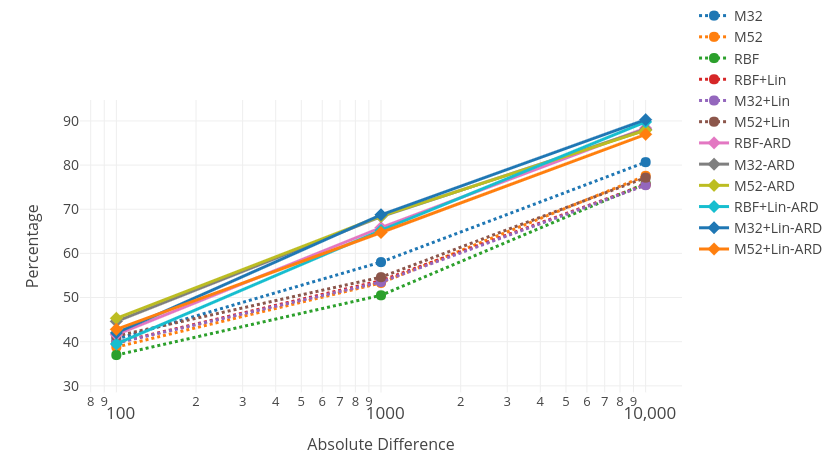
\includegraphics[width=1.0\textwidth]{ARD_diff.png}
		\caption{Absolute difference on testing set with ARD kernels. Kernels with ARD consistently give better results than kernels without ARD.}
		\label{ARD_diff}
	\end{figure}
	
	
	\subsection{Training Methods}
	Once we have chosen our kernel function, the remaining work of model selection is to optimise the $hyperparameters$ in the chosen kernel function. In this subsection, we will suppose three objective functions for training and explain how to use gradient decent based algorithm for optimisation.
	
	\subsubsection{Maximum Likelihood(ML)}
	Recall from eq. \ref{log-likelihood}, we define the marginal likelihood of training data
	\begin{equation}
	\log p(\vec y|\vec X, \vec \theta)=-\frac{1}{2}\vec y^T K_y^{-1}\vec y-\frac{1}{2}\log|K_y| - \frac{n}{2}\log 2\pi,
	\end{equation}
	where $K_y = K_{\vec f}+\sigma^2 I$ is the covariance matrix for the noisy targets value $\vec y$. $K_f$ is the covariance matrix of latent function $\vec f$ and $\sigma^2$ is the variane of i.i.d. Gaussian noise. We can interpret the first term in the marginal likelihood $-\frac{1}{2}\vec y^T K_y^{-1}\vec y$ as the data-fit since it is the only term involves target values. The second term $-\frac{1}{2}\log|K_y|$ is the complexity penalty since it only depends on the covariance matrix. The third term $- \frac{n}{2}\log 2\pi$ is the normalization constant\cite[Rasmussen and Williams, sec 5.4]{RandW}. As \textit{length-scale} increases, $K_y^{-1}$ decreases and $\log|K_y|$ increases. So we want to find a set $\vec \theta$ such that
	
	\begin{equation}
	\vec{\hat \theta} = \ \underset{\vec \theta \in \vec \Theta}{\mathrm{argmax}}\log p(\vec y|\vec X, \vec \theta).
	\end{equation}
	
	In practice, in order to find $\vec{\hat \theta}$ that maximises the log marginal likelihood, we first take partial derivatives of the the log marginal likelihood with respect to each element of the hyperparameter vector $\vec \theta$. Here, we use vector $\vec \theta$ to denote all the hyperparameters in our chosen kernel function.  Let $\vec \theta_i$ be $i^{th}$ element in $\vec \theta$, then the partial derivative of log marginal likelihood w.r.t. $\vec \theta_i$ is 
	\begin{equation}
	\begin{split}
	\frac{\partial}{\partial \vec \theta_i}\log p(\vec y|\vec X, \vec \theta) & = -\frac{1}{2}\vec y^T \frac{\partial K^{-1}}{\partial \vec \theta_i}\vec y-\frac{1}{2}\frac{\partial \log|K|}{\partial \vec \theta_i}\\
	& = -\frac{1}{2}\vec y^T\left(  -K^{-1} \frac{\partial K}{\partial \vec \theta_i} K^{-1} \right)\vec y - \frac{1}{2}\text{tr} \left(K^{-1}\frac{\partial K}{\partial\vec \theta_i}\right)\\
	&= \frac{1}{2}\vec y^TK^{-1} \frac{\partial K}{\partial \vec \theta_i} K^{-1} \vec y - \frac{1}{2}\text{tr} \left(K^{-1}\frac{\partial K}{\partial\vec \theta_i}\right)\\
	& = \frac{1}{2}\text{tr} \left( (\vec \alpha\alpha^T - K^{-1})\frac{\partial K}{\partial\vec \theta_i}\right) \text{, where } \vec \alpha = K^{-1} \vec y.
	\end{split}
	\end{equation}
	Notice that $\frac{\partial K}{\partial\vec \theta_i}$ denotes the matrix of element-wise derivatives. Then in each iteration, we update our the parameters $\vec\theta^n_i$ by
	\begin{equation}
	\vec\theta^n_i = \vec\theta^{n-1}_i - \eta\frac{\partial}{\partial \vec \theta_i}\log p(\vec y|\vec X, \vec \theta) 
	\end{equation}
	where $\eta$ is a predefined learning rate. 
	
	The main computational complexity of computing this partial derivative lies in the computing of $K^{-1}$, which is of order $\mathcal O(n^3)$ for a $n$ dimensional matrix $K$. After we have computed partial derivatives for every hyperparameters, we update each of them using a gradient decent based optimizer. Many well known packages in major programming languages have those optimizer built-in. We use Python for our implementation. One can find several more efficient optimizers such as RMSPropOptimizer and AdamOptimizer in Python. In practice, we will set our objective function to be the negative log likelihood, then we use optimizer to minimise our objective function w.r.t. hyperparameters. For those optimizers mentioned above, We can also use adaptive learning rate during optimising operation for better performance when approaching to the minimal point. By adaptive learning rate, we mean learning rate decays by a certain method. For instance, the time-based decay is specified by $\eta = \eta_0/(1+k*t)$, where $\eta_0$ is the initial learning rate, $k$ is a hyperpamater that governs the decay speed and $t$ is the iterations that have passed\cite[Bengio]{Bengio}.
	
	\subsubsection{LOO-CV Based Objective Functions}
	We can also define our objective function as the leave-one-out cross validation (LOO-CV) based predictive measure. Cross Validation (CV) based predictive measure has been successfully used in many model selection tasks in machine learning by Cawley and Talbot in \cite{Cawley_Talbot} and Sundararajan and Keerthi in \cite{Sundararajan_Keerthi}. 
	
	\subsubsection*{Geisser's surrogate Predictive Probability(GPP)}
	Predictive Sample Reuse(PSR) methods was introduced by Geisser\cite{Geisser} to be applied for both model selection and parameters optimisation problem. The basic idea is to define a partition of training data $P(N,n,\Gamma)$ such that such that $P_{N-n}^i$ is the predictive probability of $i^{th}$ subset of size $n$ in the partition. Leave-one-out cross validation is the special case when we take the size of element in the partition to be $n=1$.
	
	The predictive log likelihood when leaving out training case $i$ is
	\begin{equation}\label{GPP_1}
	\log p(y_i|\vec X,\vec y_{-i},\vec \theta) = -\frac{1}{2}\log\sigma^2_i - \frac{(y_i - \mu_i)^2}{2\sigma^2_i} - \frac{1}{2} \log 2 \pi, 
	\end{equation}
	where $\vec y_{-i}$  means all targets value except the $i^{th}$ value, $\mu_i$ and $\sigma_i$ are calculated according to eq. \ref{eq:pred4}. The training data are taken to be $(\vec X_{-i},\vec y_{-i})$. We take our objective function to be the average negative predictive log likelihood, which is given by
	\begin{equation}\label{GPP}
	\begin{split}
	G(\vec X,\vec y, \vec \theta) &= -\frac{1}{n}\sum_{i=1}^{n}\log p(y_i|\vec X,\vec y_{-i},\vec \theta)\\
	\end{split}
	\end{equation}
	This objective function is known as Geisser's surrogate Predictive Probability(GPP), first supposed by Geisser and Eddy in \cite{Geisser_Eddy}. It is also called \textit{pseudo}-likelihood by Rasmussen and Williams in \cite[sec. 5.4]{RandW}. 
	
	The main computational cost in calculating GPP is in the calculation of the predictive mean $\mu_i$ and predictive variance $\sigma^2_i$, which are dominated by the inversion of the matrix $K$ in eq. \ref{eq:pred4}. The expression for $\mu_i$ and $\sigma^2_i$ was calculated in \cite{Sundararajan_Keerthi}, and they are
	\begin{equation}\label{GPP_2}
	\begin{split}
	\mu_i &= y_i - [K^{-1}\vec y]_i/[K^{-1}]_{ii},\\
	\sigma^2_i &= 1/[K^{-1}]_{ii}.
	\end{split}
	\end{equation}
	
	Plug in these expressions into eq. \ref{GPP_1} and eq. \ref{GPP} to get the objective function. The next step is to calculate the partial derivatives of the objective function with respect to hyperparameters. We first use the expression in eq. \ref{GPP_2} to calculate the partial derivatives of the predictive mean and variance
	\begin{equation}\label{GPP_3}
	\begin{split}
	\frac{\partial\mu_i}{\partial \vec \theta_j} &= \frac{[Z_j \vec \alpha]_i}{[K^{-1}]_{ii}} - \frac{\vec \alpha_i[Z_j K^{-1}]_{ii}}{[K^{-1}]^2_{ii}},\\
	\frac{\partial\sigma^2_i}{\partial \vec \theta_j} &= \frac{[Z_j K^{-1}]_{ii}}{[K^{-1}]^2_{ii}},
	\end{split}
	\end{equation}
	where $\vec \alpha = K^{-1}\vec y$ and $Z_j = K^{-1}\frac{\partial K}{\partial \vec \theta_j}$. Using chain rule and eq. \ref{GPP_1} to calculate the partial derivatives of eq.\ref{GPP}
	\begin{equation}\label{GPP_derivative}
	\begin{split}
	\frac{\partial G(\vec X,\vec y, \vec \theta)}{\partial \vec \theta_j} &= -\frac{1}{n}\sum_{i=1}^{n}\frac{\partial \log p(y_i|\vec X,\vec y_{-i},\vec \theta)}{\partial \mu_i}\frac{\partial \mu_i}{\partial \vec \theta_j} + \frac{\partial \log p(y_i|\vec X,\vec y_{-i},\vec \theta)}{\partial \sigma^2_i}\frac{\partial \sigma^2_i}{\partial \vec \theta_j}\\
	&=-\frac{1}{n}\sum_{i=1}^{n}\left(\alpha_i[Z_j \vec{\alpha}]_i - \frac{1}{2}\left(1+\frac{\alpha^2_i}{[K^{-1}]_{ii}}\right)[Z_j K^{-1}]_{ii}\right)/[K^{-1}]_{ii}.
	\end{split}
	\end{equation}
	
	With partial derivatives calculated, we can use gradient decent based optimizer to minimise our objective function $G(\vec X,\vec y, \vec \theta)$, thus find the optimal $\hat{\vec\theta}$ such that
	
	\begin{equation}
	\vec{\hat \theta} = \ \underset{\vec \theta \in \vec \Theta}{\mathrm{argmax}}G(\vec X,\vec y, \vec \theta).
	\end{equation}
	
	\subsubsection*{Geisser's Predictive mean square Error (GPE)}
	Another LOO-CV based objective function is Geisser's Predictive mean square Error (GPE)\cite[Geisser and Eddy]{Geisser_Eddy}\cite[Sundararajan and Keerthi]{Sundararajan_Keerthi}. GPE is define by
	\begin{equation}
	\frac{1}{n}\sum_{i=1}^{n}\mathbb E[(y_i-\hat{y}_i)^2], 
	\end{equation}
	where $\hat{y}_i$ is the predicted value from the model using data set $(\vec X_{-i}.\vec y_{-i})$ and $y_i$ is the true target value. GPE measures the average expected square error derived from LOO-CV. The objective function corresponding to GPE is
	\begin{equation}\label{GPE}
	\begin{split}
	G_E(\vec X,\vec y, \vec \theta) = \frac{1}{n}\sum_{i=1}^{n}\int (y_i-\hat{y}_i)^2 p(\hat y_i|\vec X,\vec y_{-i},\vec \theta)d\hat y_i,
	\end{split}
	\end{equation}
	where $\hat y_i$ follows a Gaussian distribution with mean $\mu_i$ and variance $\sigma^2_i$ given by eq. \ref{GPP_2}. Thanks to the analytical tractability of Gaussian distribution, we can simplify the objective function as 
	\begin{equation}\label{GPE_1}
	G_E(\vec X,\vec y, \vec \theta) = \frac{1}{n}\sum_{i=1}^{n}(y_i-\mu_i)^2+\sigma^2_i.
	\end{equation}
	We can see from the expression of $G_E$, this objective function will aim to minimise the deviation between the predictive mean and the true value as well as the predictive variance. In the most ideal case, $G_E$ should be very closed to zero, meaning that expected error of training set derived based on LOO-CV should be very small. 
	
	We can also use chain rule and eq. \ref{GPP_1} to calculate the partial derivatives of GPE objective function
	\begin{equation}\label{GPE_derivative}
	\frac{\partial G_E(\vec X,\vec y, \vec \theta)}{\partial \vec \theta_j} = \frac{1}{n}\sum_{i=1}^{n}\frac{\partial (y_i-\mu_i)^2}{\partial \mu_i}\frac{\partial \mu_i}{\partial \theta_j}+2\sigma_i\frac{\partial \sigma_i}{\partial \theta_j}.
	\end{equation}
	Plug in eq. \ref{GPP_3} to get
	\begin{equation}\label{GPE_derivative_2}
	\frac{\partial G_E(\vec X,\vec y, \vec \theta)}{\partial \vec \theta_j} = \frac{1}{n}\sum_{i=1}^{n}\left([Z_j K^{-1}]_{ii}\left(1+2\frac{\vec\alpha^2_i}{[K^{-1}]_{ii}}\right)-2\vec \alpha_i[Z_j\vec\alpha]_i\right)/[K^{-1}]_{ii},
	\end{equation}
	where $\vec \alpha = K^{-1}\vec y$ and $Z_j = K^{-1}\frac{\partial K}{\partial \vec \theta_j}$.
	
	Once we have calculated the partial derivatives, we will follow the similar steps in the maximum likelihood case to find the optimal $hyperparameter$ $\hat{\vec \theta}$ such that
	\begin{equation}
	\vec{\hat \theta} = \ \underset{\vec \theta \in \vec \Theta}{\mathrm{argmax}}G_E(\vec X,\vec y, \vec \theta).
	\end{equation}
	
	The main difference is that maximum likelihood gives us the probability of training data given the assumption of model while the two LOO-CV based methods estimate the predictive probability and error which gives us a measure of how good our assumption is. 

\subsubsection{Numerical Results}\label{subsec:num_res}
	The three objective proposed above have similar computational expense, all dominated by the inversion of covariance matrix $K$, which is $\mathcal O(n^3)$. However, the two LOO-CV based methods have additional $\mathcal O(n^2)$ cost for the entire process of calculating the predictive probability and error. This difference will emerge when the train set is large and when we run a large number of iterations. For 4 batches of 2048 points each, ML takes about one third less time compared to the two LOO-CV based methods. Exact numbers are in Table \ref*{training_time}.
	
	Table \ref*{multitrain_rbf}, \ref{multitrain_matern32} and \ref{multitrain_matern52} show that results from these three methods vary between different kernels. For the data set we are using, the best performance comes from the GPP method with Mat\'ern32 kernel, which is consistent with results from Table \ref{table:res_single_lengthscale} and \ref{ARD_res}. Out of the three methods, the GPE method is consistently the worst performer with all kernels. We can explain this result by reparameterizing the objective function $G_E(\vec X,\vec y, \vec \theta)$. 
	
	We can start by denote the covariance matrix by $K = \sigma^2 \bar K$, where $\sigma$ is a variance parameter. Then we have $\bar K^{-1} = \sigma^2 K^{-1} $. By eq. \ref{GPP_2} and \ref{GPE_1}, we get the reparameterized GPE objective function
	\begin{equation}\label{reparameterized_GPE}
	\begin{split}
	G_E(\vec X,\vec y, \vec \theta) &= \frac{1}{n}\sum_{i=1}^{n}(y_i-\mu_i)^2+\frac{1}{n}\sum_{i=1}^{n}\sigma^2_i\\
	& = \frac{1}{n}\sum_{i=1}^{n}\left(\frac{[K^{-1}\vec y]_i}{[K^{-1}]_{ii}}\right)^2+\frac{1}{n}\sum_{i=1}^{n}\frac{1}{[K^{-1}]_{ii}}\\
	& = \frac{1}{n}\sum_{i=1}^{n}\left(\frac{[\bar K^{-1}\vec y]_i}{[\bar K^{-1}]_{ii}}\right)^2+\frac{\sigma^2}{n}\sum_{i=1}^{n}\frac{1}{[\bar K^{-1}]_{ii}}.
	\end{split}
	\end{equation}
	Since $\sigma$ is independent of $\bar K$, when we minimise the objective function, $\sigma$ will be pushed towards zero. Then the covariance matrix $K$ will be pushed towards zero too, which is not true\cite{Sundararajan_Keerthi}. This is why results from GPR are bad for all kernel functions.
	
	\begin{table}
		\centering
		\begin{tabular}{c|cccc|cccc} 
			\toprule
			& \multicolumn{4}{l|}{Training data absolute difference}            & \multicolumn{4}{l}{Testing data absolute difference~ ~ ~}          \\
			& 10             & 100            & 1000           & 10000          & 10             & 100            & 1000           & 10000           \\ 
			\hline\hline
			ML  & \textbf{47.94} & \textbf{74.13} & \textbf{94.06} & \textbf{99.96} & \textbf{27.45} & \textbf{41.58} & \textbf{65.83} & \textbf{88.38}  \\
			GPP & 42.86          & 68.66          & 89.23          & 99.89          & 24.45          & 38.28          & 60.72          & 85.57           \\
			GPE & 15.25          & 31.98          & 60.23          & 81.73          & 13.03          & 26.55          & 52.40          & 77.86           \\
			\bottomrule
		\end{tabular}
		\caption{Different training methods  for RBF kernel}
		\label{multitrain_rbf}
	\end{table}
	
	\begin{table}
		\centering
		\begin{tabular}{c|cccc|cccc} 
			\toprule
			& \multicolumn{4}{l|}{Training data absolute difference}              & \multicolumn{4}{l}{Testing data absolute difference~ ~ ~}           \\
			& 10              & 100             & 1000           & 10000          & 10              & 100            & 1000           & 10000           \\ 
			\hline\hline
			ML  & 58.51           & 83.42           & \textbf{98.35} & \textbf{99.98} & 30.76           & \textbf{44.59} & \textbf{68.34} & \textbf{88.08}  \\
			GPP & \textbf{63.22 } & \textbf{83.58 } & 97.64          & 99.83          & \textbf{31.56 } & 43.59          & 64.03          & 84.97           \\
			GPE & 17.57           & 36.76           & 65.73          & 85.42          & 14.03           & 29.46          & 54.91          & 79.26           \\
			\bottomrule
		\end{tabular}
		\caption{Different training methods for Matern32 kernel}
		\label{multitrain_matern32}
	\end{table}
	
	\begin{table}
		\centering
		\begin{tabular}{c|cccc|cccc} 
			\toprule
			& \multicolumn{4}{l|}{Training data absolute difference}            & \multicolumn{4}{l}{Testing data absolute difference~ ~ ~}          \\
			& 10             & 100            & 1000           & 10000          & 10             & 100            & 1000           & 10000           \\ 
			\hline\hline
			ML  & \textbf{56.10} & \textbf{81.23} & \textbf{97.52} & \textbf{99.98} & 29.56          & \textbf{45.29} & \textbf{68.44} & \textbf{87.88}  \\
			GPP & 57.65          & 78.82          & 96.00          & 99.88          & \textbf{30.36} & 40.98          & 62.73          & 84.77           \\
			GPE & 29.24          & 57.01          & 78.88          & 95.47          & 20.24          & 36.77          & 59.12          & 83.77           \\
			\bottomrule
		\end{tabular}
		\caption{Different training methods  for Matern52 kernel}
		\label{multitrain_matern52}
	\end{table}
	
	\begin{table}
		\centering
		\begin{tabular}{c|ccc} 
			\toprule
			& RBF   & Matern32 & Matern52  \\ 
			\hline\hline
			ML  & 5.89s & 5.70s    & 5.93s     \\
			GPP & 9.01s & 8.85s    & 8.79s     \\
			GPE & 9.14s & 9.04s    & 8.92s     \\
			\bottomrule
		\end{tabular}
		\caption{Training time per iteration of entire dataset from different methods. Algorithm is implemented using Python 3.5 and Tensorflow packge. Run on machine with CPU: Intel Xeon E5-2620 v4 2.10GHz, RAM: 32.0GB.}
		\label{training_time}
	\end{table}
	
	
	\newpage
	\section{Data Analysis}\label{sec:data_analysis}
	
	\subsection{Data Description}
	The data used during implementation is propriety data from Citigroup. The feature space contains $1290$ dimensions of numeric values and the target value is the price of synthetic CDO. Since all feature dimensions are numeric, this paper will not discuss handling with missing features and converting non-numerical features to numeric features. After removing feature dimensions with variance less than $0.01$\footnotemark[3], there are still $1118$ dimensions left. Within some of these dimensions, there are large differences between the minimum and maximum values. So before doing any specific data processing, one should first rescale all feature dimensions into the interval of $[0,1]$ for better computational performance. By rescaling all dimensions into uniform interval, it can effectively avoid model misspecification because of large difference in numeric ranges of feature values\cite{Kotsiantis}. Another benefit of rescaling all feature values into uniform interval lies in the more reasonable initialization of parameters.  The \textit{characteristic length-scale} in kernel functions can be conveniently initialized to be $0.5$ or $1.0$ for all dimensions, then perform optimization. After doing this pre-processing, the remaining section will be focused on dimension reduction techniques.	
	\footnotetext[3]{
		The variance of a random variable measures how far a set of observations are spread out from the mean. A constant random variable has zero variance. By removing dimensions with near zero variance, we discard those dimensions that are almost constant in all data points. 
	}
	
	\subsection{Dimension Reduction}
	Due to the computational expense of calculating the inverse of covariance matrix, which is of order $\mathcal O(n^3)$ for a $n$-dimensional positive semi-definite matrix, it is hard to work with large data set in practice. However, for high dimensional input, one must train the model with a reasonably large amount of data so that on average each dimension is adequately represented. Also, as mentioned above, one has to optimize more parameters for high dimension data if using ARD kernels. This also requires training the model with a large amount of data for parameters to converge. But it is restricted by $\mathcal O(n)$ computational complexity of covariance matrix inversion. To tackle this dilemma, one needs to reduce the dimension of feature space while retaining the information from the original data. In this subsection, two dimension reduction techniques will be presented, namely Principal Component Analysis(PCA) and Autoencoder(AE). 
	
	\subsubsection{Principal Component Analysis}
	Principal Component Analysis(PCA) is used extensively in statistics for data representation and dimension reduction. The main purpose of PCA is to find a new coordinate system in which we can express the original data with less dimensions without significant loss of information. The following paragraph will briefly explain how PCA works. For a detailed discuss about PCA, please see \cite[Jolliffe]{Jolliffe}.
	
	To perform PCA, one will first need to standardize the data by subtracting mean and dividing standard deviation. Then calculate the sample covariance matrix of the input data $\vec Q = \frac{1}{n-1}\vec X\vec X^T$, where each column of $\vec X$ is one data point in original input space, $\mathbb R^d$. Then find the eigenvalues $\lambda_1, \cdots,\lambda_d$ of $\vec Q$ and corresponding orthogonal eigenvectors $\vec u_1,\cdots,\vec u_d$. Once all the eigenvalues have been calculated, one needs to sort the eigenvalues in descending order and corresponding eigenvectors. The eigenvector corresponding to the largest eigenvalue is called first \textit{principal component} and so on. To reduce dimensions, one discards those eigenvectors corresponding to eigenvalues that are smaller than a predefined threshold(small eigenvalues correspond to eigenvectors containing less information about the original data). One can also precede by choosing the first $d$ eigenvalues until
	\begin{equation}
	\frac{\sum_{i=1}^{k}\lambda_i}{\sum_{j=1}^{d}\lambda_j}\geq \epsilon, 
	\end{equation} 
	where $\epsilon$ is the percentage of variance one wants to keep from the original data. Now there are $k$($<d$) eigenvectors to form the feature matrix $\vec U$ which is of shape $k\times d$. The dimension reduction is done by multiplying $\vec X$ by $\vec U$ from left,
	\begin{equation}
	\vec X' = \vec U \cdot \vec X
	\end{equation}
	where $\vec X'$ is a $k\times n$ matrix with each column a transformed data point in reduced input space $\mathbb R^k$.
	
	\subsubsection{Autoencoder}
	An autoencoder is a type of feed forward neural network that is mainly used for efficient data encoding\cite[chapter 14]{Deep_Learning}. The most simple case of autoencoder contains three layers -- namely, input layer, hidden layer and output layer. This type of autoencoder can be divided into two parts: an encoder function and a decoder function. An encoder function takes the original data as input and transform it to a transformed space. Denote the encoder as $\vec h = f(\vec x)$, where $\vec x\in \mathbb R^d, \vec h\in \mathbb R^m$. A decoder function takes $\vec h$ as input and outputs a reconstruction of the original data $\vec x' = g(\vec h)$, where $\vec x'\in \mathbb R^d$. One can train the model by minimize the reconstruction error between $\vec x$ and $\vec x'$. Commonly used reconstruction error measure is the Mean Squared Error loss function 
	\begin{equation}
	L(\vec x,\vec x') = \frac{1}{n}\sum_{i=1}^{n}(\vec x_i-\vec x'_i)^2. 
	\end{equation}
	\begin{figure}[h!]
		\centering
		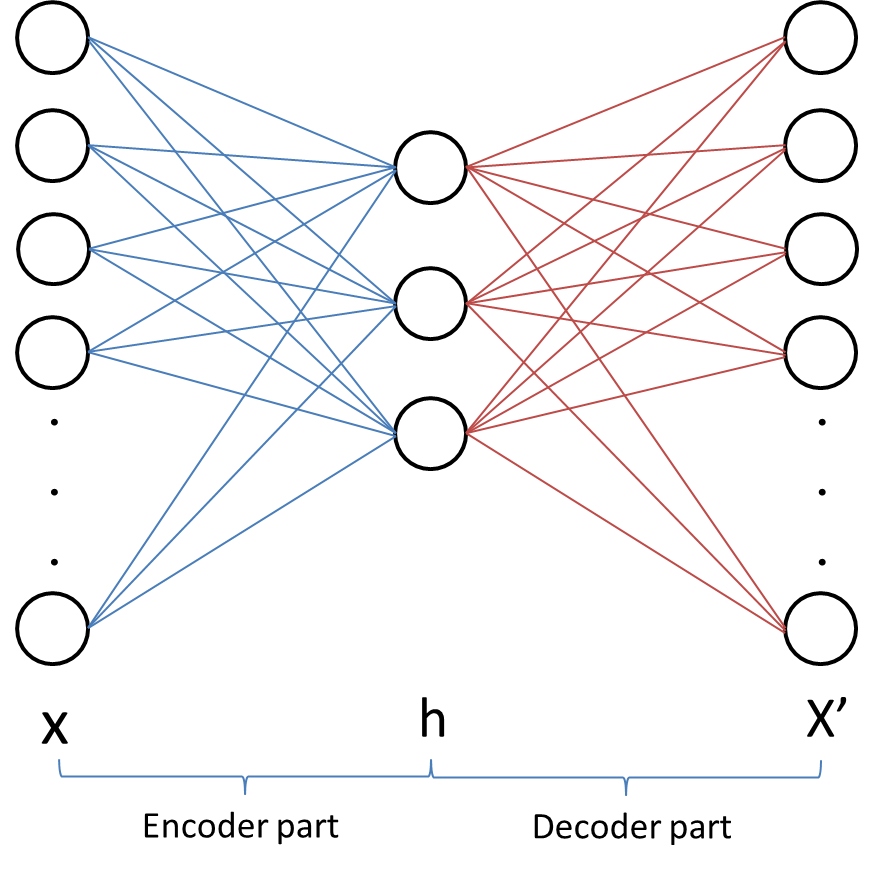
\includegraphics[width=0.5\textwidth]{ae.png}
		\caption{Undercomplete Autoencoder Training Scheme. In an undercomplete autoencoder, number of neurons in the hidden layer is smaller than the number of input dimension.}
	\end{figure}

	
	When $m<d$, it means the encoder function transforms the original data into a lower dimensional space and the decoder function can recover the original data from the transformed space within a tolerable error range. This type of autoencoders is called \textit{undercomplete autoencoders}(hidden layer dimension fewer than input dimension) and is widely used as a dimension reduction tool. By setting the hidden layer size smaller than the input dimension and minimizing the reconstruction error, it forces the autoencoder to learn meaningful transformation of original features.
	When the activation function used in the encoder part is linear, i.e. $f(\vec x) = \vec w\cdot\vec x + b$, and the hidden layer is fully connected, the subspace spanned by the autoencoder by the encoder function is the same as the one spanned by principal components from PCA. Detailed discussion and proof are provided by Plaut in \cite{Plaut}.
	

	
	When the activation function is non-linear, e.g. the logistic function
	\begin{equation}
	\begin{split}
	f(\vec x) &= \frac{1}{1+\exp[-(\vec w\cdot\vec x + b)]},\\
	g(\vec h) &= \frac{1}{1+\exp[-(\vec w'\cdot\vec h + b')]},
	\end{split}
	\end{equation}
	where $\vec w, b$ and $\vec w', b'$ are weights and bias of the encoder and decoder function, the autoencoder can learn a more useful non-linear generalization of the one generated by PCA. 
	After the training process, one can discard the decoder part and only apply the encoder function to the whole data set for dimension reduction purpose.
	
	
	
	Apart from dimension reduction, one can also add denoising feature to the autoencoder by feed the model with \textit{noisy} data, then try to reconstruct the \textit{clean} data. This type of autoencoders are called \textit{denoising autoencoders}. 
	
	In a denoising autoencoder, a random noise, usually Gaussian noise, is added to the original data $\vec y$ to get noisy data $\hat{\vec y}$. Then apply the encoder function and decode function to get $\hat{\vec h} = f(\vec y)$  and $\vec{\hat y'} = g(\hat{\vec h})$. The loss function is defined as Mean Squared Error between the reconstructed $\vec{\hat y'}$ and the original data $\vec y$. The training process it to minimize $L(\vec y,\vec{\hat y'})$. 
	
	\begin{figure}[h!]
		\centering
		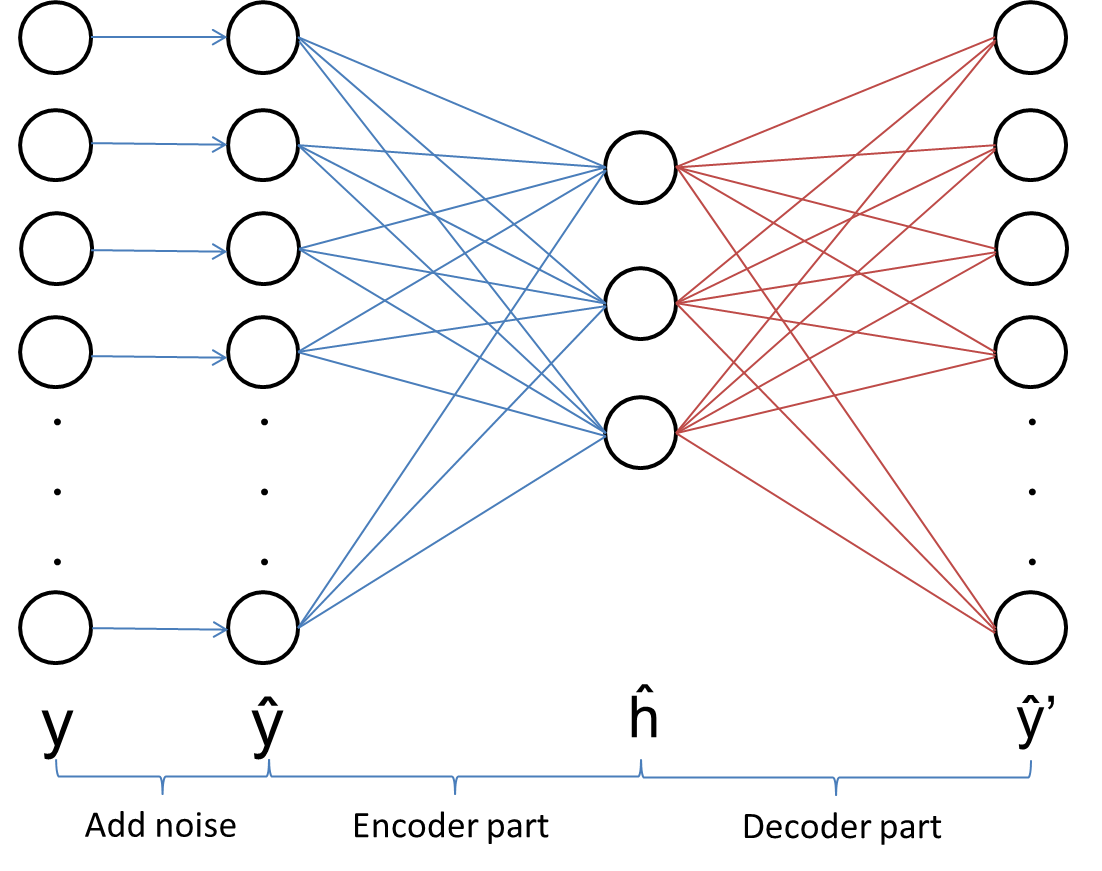
\includegraphics[width=0.65\textwidth]{dae.png}
		\caption{Denoising Autoencoder Training Scheme. Manually add noise to the original data before feeding into the AE.}
	\end{figure}
	
	\subsection{Numerical Results}\label{sec:data_ana_res}
	While traditional dimension reduction techniques like PCA are methods, undercomplete autoencoder is a family of methods. One can configure different autoencoders by number of nodes in the hidden layer or number of hidden layers. One can immediate see this can go on forever. Like the configuration of a normal Neural Network, the configuration of an undercomplete autoencoder for a specific dataset is often based on experience and experiments. For computational tractability, the implementaion will use only one hidden layer in this paper. The hidden layer is set to be a dense layer, which means every nodes in a layer is fully connected to every nodes from the previous layer. The empirically-derived rule-of-thumb for sizes of hidden layers is $2^n$. In this implementation, it starts with 256 nodes, approximately one-fourth of the original dimension and gradually decrease to 16. Training results for autoencoders with different sizes are shown in the following figures.
	\begin{figure}[h!]
		\centering
		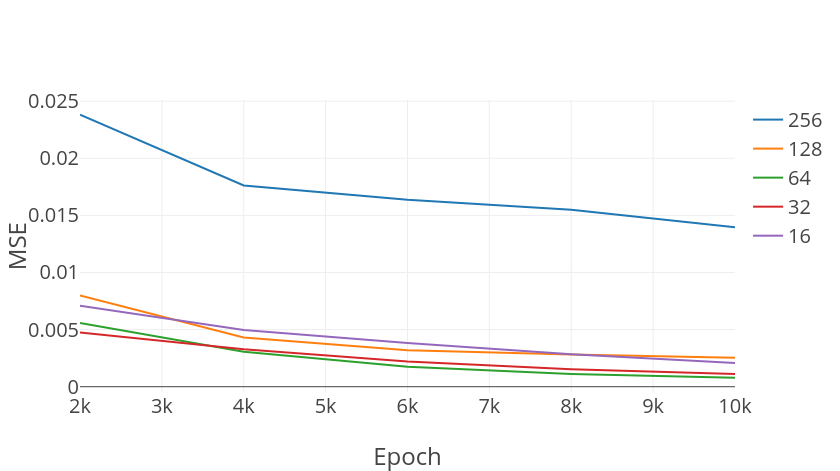
\includegraphics[width=.8\textwidth]{ae_mse.png}
		\caption{Training Process of Different AE Size. All sizes converge at similar speed, the MSE differences between 4000 and 10000 iterations are subtle. AEs with fewer hidden nodes(128,64,32,16) are able to reconstruct the original data with less error than AE with 256 hidden nodes.}
		\label{ae_res}
	\end{figure}
	
	\begin{figure}[h!]
		\centering
		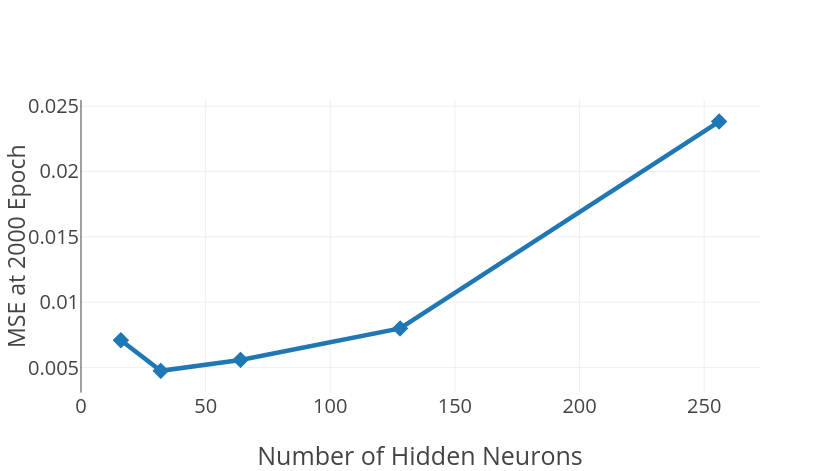
\includegraphics[width=.8\textwidth]{ae_compare.png}
		\caption{Training Results at 2000 Epochs. Reconstuction error is at lowest when the AE has 32 hidden nodes. }
		\label{ae_res_1}
	\end{figure}
	
	From figure \ref{ae_res} and \ref{ae_res_1}, when further compressing the data to lower dimension, the AE is actually able to reconstruct the original data within smaller error range. This means the AE with non-linear activation function can effectively learn meaningful features in a much lower dimensional space that can recover the original information within little error. 
	
	Feed the reduced data into our GPR model with RBF kernel and Matern32 kernel. Results from differnt methods are shown in table \ref{dim_red_res}. Consistently with previous results, Matern32 kernel continues to outperform the RBF kernel in all reduced data set. This means that indexed by the reduced feature space, our target function is still not smooth enough to be modeled by a GP with RBF kernel. The column $PCA99\%$ means the PCA remains $99\%$ of the variance from the original data when performing PCA, which will reduce feature dimensions to $225$. The results from $PCA99\%$ is worse than those from AE with different sizes. This is because PCA only performs linear transformation from the original feature space to the reduced space. For the data set we use, the reduced space from PCA method does not contain as much information as those spanned from AEs. On the other hand, the non-linear activation function embedded in AEs is able to learn useful non-linear transformation from the original feature space that can be used to reconstruct the original information with little error. Results from GPR prediction shows that this non-linear transformation does not necessarily benefit from the increasing in the number of hidden nodes. This means for the used data set, non-linear mapping into a smaller space is able to retrain more information than a larger one. For the AEs used, the one with 64 hidden nodes performs the best.
	 
	
	\begin{sidewaystable}
		\centering
		\scalebox{0.98}{\begin{tabular}{c|c|cc|cc|cc|cc|cc|cc} 
				\toprule
				\multicolumn{1}{c}{}                                                                              &       & \multicolumn{2}{c|}{256} & \multicolumn{2}{c|}{128} & \multicolumn{2}{c|}{64} & \multicolumn{2}{c|}{32} & \multicolumn{2}{c|}{16} & \multicolumn{2}{c}{PCA 99\%}  \\ 
				\cline{3-14}
				\multicolumn{1}{c}{}                                                                              &       & RBF   & Matern32         & RBF   & Matern32         & RBF   & Matern32        & RBF   & Matern32        & RBF   & Matern32        & RBF   & Matern32              \\ 
				\hline\hline
				\multirow{4}{*}{\begin{tabular}[c]{@{}c@{}}Training \\data \\absolute \\difference \end{tabular}} & 10    & 31.31 & 16.60            & 32.60 & 57.17            & 34.63 & 58.73           & 24.17 & \textbf{58.85}  & 41.27 & 54.43           & 22.68 & 23.08                 \\
				& 100   & 54.31 & 37.51            & 57.07 & 77.45            & 58.70 & \textbf{79.28}  & 54.04 & 78.80           & 64.00 & 75.99           & 48.24 & 51.97                 \\
				& 1000  & 76.39 & 64.70            & 78.34 & 93.46            & 79.50 & \textbf{94.82}  & 74.44 & 94.48           & 84.00 & 91.38           & 69.51 & 71.11                 \\
				& 10000 & 91.82 & 82.24            & 92.49 & 98.88            & 93.85 & 98.90           & 92.04 & 98.82           & 94.53 & \textbf{99.24}  & 88.39 & 87.71                 \\ 
				\hline
				\multirow{4}{*}{\begin{tabular}[c]{@{}c@{}}Testing \\data \\absolute \\difference \end{tabular}}    & 10    & 18.22 & 10.49            & 18.95 & 26.59            & 18.03 & \textbf{26.77}  & 12.88 & 25.94           & 20.42 & 24.75           & 12.83 & 13.43                 \\
				& 100   & 30.63 & 23.46            & 33.58 & \textbf{39.56}   & 33.21 & 38.64           & 27.69 & 39.28           & 32.38 & 37.63           & 28.59 & 27.60                 \\
				& 1000  & 52.25 & 39.56            & 54.00 & 60.07            & 53.54 & \textbf{60.07}  & 47.01 & 57.96           & 49.68 & 56.30           & 47.29 & 45.45                 \\
				& 10000 & 78.29 & 72.59            & 77.92 & 81.14            & 78.29 & 80.40           & 76.91 & \textbf{82.34}  & 77.09 & 80.13           & 75.08 & 72.68                 \\
				\bottomrule
			\end{tabular}}
			\caption{Autoencoder and PCA results of RBF and Matern32 kernels; the numbers, 128, 64, ..., mean the number of neurons in the hidden layer of an undercomplete autoencoder. PCA 99\% means sum of chosen eigenvalues is 99\% of the sum of total eigenvalues. Results from AEs are consistently better than those from PCA. This means linear transformation used in PCA is not able to retain as much information as non-linear transformation in AEs. Adding the hidden nodes in AE does not necessarily improve prediction performance from GPR model.}
			\label{dim_red_res}
		\end{sidewaystable}
		
		%	\newpage
		%	
		%	\section{Relationships between GPR and Other Models}
		%	
		%	\subsection{Representer Theory}
		%	
		%	\subsection{Radial Basis Function Network}
		
		\newpage
		\section{Conclusion, Discussion and Further Study}
		
		This section will wrap up what has been shown in previous sections and discuss other applications of GP for further study.
		
		This paper starts with brief introduction to pricing formulas for synthetic CDO -- a structured credit product. Then it proposes an alternative way of replicating prices using a Bayesian learning model -- Gaussian Process Regression. In section 2, it has shown Gaussian process from a extended weight-space view and a more intuitive function-space view. For a zero mean Gaussian process as proposed in this paper, the behaviour of the GP is fully specified by its covariance matrix produced by kernel functions. There are numerous choices for kernels function. Section 3 has discussed three stationary kernel functions namely, Radial Basis Function(RBF) and Mat\'ern family kernel functions(Mat\'ern32 and Mat\'ern52), and one non-stationary kernel function -- Linear kernel function. Section 3 has also proposed three objective functions for parameter optimization -- namely, Maximum Likelihood(ML), Geisser's surrogate  Predictive Probability(GPP) and Geisser's Predictive mean square Error(GPE). In terms of computation complexity, ML objective functions requires less time for each iteration during training than other two objective functions. Numerical results are shown in Section \ref{subsec:num_res}. For the used dataset, Mat\'ern32 kernel function combined with GPP objective function gives the best predictive results.
		
		The expensive computational complexity($\mathcal O(n^3)$) of GPR model during training process prohibits us from using a larger, more representative data set. To tackle this problem, we have used two dimension reduction techniques -- namely, Principal Component Analysis(PCA) and Autoencoder(AE) and compared the results on our dataset in Section \ref{sec:data_ana_res}. When applying the reduced data to our GPR model, results from AEs with different number of hidden nodes are consistently better than those from PCA. This is because the non-linear transformation performed by the activation function of AEs can produce a reduced space retaining more meaningful information from the original dataset than  the linear transformation in PCA.
		
		The autoencoder is a family of methods. One can construct complex hidden layers and nodes configuration as well as training loss function when dealing with a specific data set. For computational tractability, this paper has used one dense hidden layer for the implementation. However, one can build an autoencoder tailored for a specific data set for better performance. 
		
		It has been shown in Section \ref{subsec:kernel_func} that sample paths of GPs governed by a Mat\'ern32 kernel function are rougher than those by a RBF kernel function. Prediction results also validate that Mat\'ern32 kernel performs better than RBF kernel on our dataset. However, when applied to a another dataset, one needs to first analyse the distribution of features and the behaviour of the target function so that one can construct a suitable kernel function. It is also worth exploring that different kernel functions can be applied to different dimensions of the feature space, based on their different distribution and the smoothness of target values with respect to that dimension.
		
		Since differentiation is a linear operation, the derivative of a Gaussian process is another Gaussian process. Thus one can model the derivative of the target function as a GP and make inference from that. This can be applied to model underlyings of a structured or exotic products for hedging and risk management purposes. The covariance of partial derivative with function value and covariance between partial derivatives can be specified by the kernel function $k$ in the following form
		\begin{equation}
		\begin{split}
		\text{cov}\left(f_i,\frac{\partial f_j}{\partial x_{d_j}}\right)&=\frac{\partial k(\vec x_i,\vec x_j)}{\partial x_{d_j}}\\
		\text{cov}\left(\frac{\partial f_i}{\partial x_{d_i}},\frac{\partial f_j}{\partial x_{d_j}}\right)&=\frac{\partial^2 k(\vec x_i,\vec x_j)}{\partial x_{d_i}\partial x_{d_j}},
		\end{split}
		\end{equation}
		where $d_j$ denotes the $j^{th}$ dimension in the feature space. If certain dimensions in the feature space are of interest, one can just remove columns in the covariance matrix that are irrelevant. Inference and predictions when modelling with partial derivative are done similarly to the procedure described in this paper.
		%deep Gaussian process
		
		%combine GPR and Kalman Filter, use GPR to produce measure and variance for hidden state estimation update in kalman filter
		
		
		
		
		%%%%%%%%%%%%%%%%%%%%%%%%%%%%%%%%%%%%%%%%%%%%%%%%%%%%
		
		%
		%\section{How to write mathematics}\label{sec:HowTo}
		%In this section, we show some examples of properly written mathematical expressions and sentences.
		%In the header of your thesis, you can define \LaTeX \ shortcuts to write more quickly.
		%
		%
		%
		%%%%%%%%%%%%%%%%%%%%%%%%%%%%%%%%%%%%%%%%%%%
		%\subsection{The Black-Scholes model}
		%Consider a given probability space $(\Omega, \mathcal{F},\mathbb{P})$ 
		%supporting a Brownian motion~$(W_t)_{t\geq 0}$.
		%In the Black-Scholes model, the stock price process~$(S_t)_{t\geq 0}$ is the unique strong solution to
		%the following stochastic differential equation:
		%\begin{equation}\label{eq:BS}
		%\frac{\D S_t}{S_t} = r \D t + \sigma \D W_t,
		%\qquad S_0>0,
		%\end{equation}
		%where $r\geq 0$ denotes the instantaneous risk-free interest rate and $\sigma>0$ the instantaneous volatility.
		%A European call price $C_t(S_0,K,\sigma)$ with maturity $t>0$ and strike $K>0$ 
		%pays at maturity $(S_t-K)_+=\max(S_t-K,0)$. 
		%When the stock price follows the Black-Scholes SDE~\eqref{eq:BS}, 
		%Black and Scholes~\cite{BS73} proved that its price at inception is worth
		%$$
		%C_t(S_0,K,\sigma) = S_0\mathcal{N}(d_+) - K\E^{-rt}\mathcal{N}(d_-),
		%$$
		%where
		%$$
		%d_{\pm} := \frac{\log\left(S_0 \E^{rt}/K\right)}{\sigma\sqrt{t}} \pm \frac{\sigma\sqrt{t}}{2},
		%$$
		%and where~$\mathcal{N}$ denotes the cumulative distribution function of the Gaussian random variable.
		%
		%
		%
		%%%%%%%%%%%%%%%%%%%%%%%%%%%%%%%%%%%%%%%%%%%
		%\subsection{Inserting a picture}
		%Here are some examples of how to insert a picture:
		%
		%\begin{figure}[!ht]
		%\centering
		%\subfigure{\includegraphics[scale=0.2]{Picture.eps}}
		%\caption{This is the caption for the figure, detailing what the figure represents.
		%Parameter values,...}
		%\label{fig:Pict}
		%\end{figure}
		%
		%\begin{figure}[!ht]
		%\centering
		%\subfigure{\includegraphics[scale=0.3]{Picture.eps}}
		%\hspace{15pt}
		%\subfigure{\includegraphics[scale=0.3]{Picture.eps}}
		%\caption{Another caption.}
		%\label{fig:Pict2}
		%\end{figure}
		%
		%
		%
		%%%%%%%%%%%%%%%%%%%%%%%%%%%%%%%%%%%%%%%%%%%
		%\subsection{More complicated mathematical expressions}
		%In the Heston model, the stock price is the unique strong solution to the following stochastic differential equation:
		%\begin{equation}\label{eq:Heston}
		%\begin{array}{rll}
		%\D S_t & = S_t \sqrt{V_t} \D W_t, & S_0 = s>0,\\
		%\D V_t & = \kappa(\theta-V_t)\D t + \xi\sqrt{V_t}\D Z_t, & V_0 = v_0>0,\\
		%\D \langle W, Z\rangle_t & = \rho \D t,
		%\end{array}
		%\end{equation}
		%where $\kappa, \xi, \theta, v_0, s>0$ and the correlation parameter $\rho$ lies in $[-1,1]$.
		%In the system~\eqref{eq:Heston}, the process $(V_t)_{t\geq 0}$ represents the instantaneous
		%variance (squared volatility) of the underlying stock price~$S$.
		%Existence of a unique strong solution for the variance process (also called the Feller process)
		%are guaranteed by the Yamada-Watanabe conditions~\cite[Proposition 2.13, page 291]{KS97}). 
		%
		%
		%%%%%%%%%%%%%%%%%%%%%%%%%%%%%%%%%%%%%%%%%%%
		%\subsection{Writing Definitions, Theorems,...}
		%All the environments for Definitions, Theorems,... are already defined in \LaTeX. 
		%Here is an example:
		%\begin{theorem}[Static replication]\label{thm:StaticReplication}
		%Let~$f:\RR\to\RR$ be a $\mathcal{C}^2$ function, and $F$ a non-negative constant.
		%A European option with payoff $f(S)$ can be fully statically replicated using only cash, 
		%the underlying stock and a continuum of European Calls and Puts.
		%\end{theorem}
		%\begin{proof}
		%By the fundamental theorem of calculus, we have
		%\begin{align*}
		%f(S) & = f(F) + \ind_{\{S>F\}}\int_F^S f'(u)\D u  \ - \  \ind_{\{S<F\}}\int_S^F f'(u)\D u \\
		% & = f(F) + \ind_{\{S>F\}}\int_F^S\left[f'(F) + \int_F^u f''(v)\D v\right]\D u
		% - \ind_{\{S<F\}}\int_S^F \left[f'(F) - \int_u^F f''(v) \D v\right]\D u\\
		% & = f(F) + f'(F) (S-F) + \ind_{\{S>F\}}\int_F^S \int_v^S f''(v)\D u \D v  + \ind_{\{S<F\}}\int_S^F \int_S^v f''(v)\D v\D u \\
		% & = f(F) + f'(F) (S-F) + \ind_{\{S>F\}}\int_F^S f''(v)(S-v) \D v  + \ind_{\{S<F\}}\int_S^F f''(v) (v-S)\D v \\
		% & = f(F) + f'(F) (S-F) + \ind_{\{S>F\}}\int_F^\infty f''(v)(S-v)_+ \D v  + \ind_{\{S<F\}}\int_0^F f''(v) (v-S)_+ \D v
		%\end{align*}
		%\end{proof}
		%
		%\begin{remark}
		%The following two special cases of Theorem~\ref{thm:StaticReplication} are of particular financial importance:
		%\begin{itemize}
		%\item if $F=0$, then the expression above reduces to 
		%$$
		%f(S) = f(0) + S f'(0) + \int_F^\infty f''(v)(S-v)_+ \D v, 
		%$$
		%which means that the option with payoff $f(S)$ can be replicated by $f(0)$ invested in bonds, $f'(0)$ shares 
		%and an infinite strip of call options, each with strike~$v$ and in quantity~$f''(v)$;
		%\item if $F=S_0$, then the formula above reads
		%$$
		%f(S) = \left[f(S_0) - S_0 f'(S_0) \right] + S f'(S_0) + \ind_{\{S>S_0\}}\int_{S_0}^\infty f''(v)(S-v)_+ \D v
		% \ + \ \ind_{\{S<S_0\}}\int_0^{S_0} f''(v)(v-S)_+ \D v\D u,
		%$$
		%so that the option with payoff $f(S)$ can be replicated with bonds, stocks and European Calls and Puts.
		%\end{itemize}
		%\end{remark}
		%
		%
		%
		%%%%%%%%%%%%%%%%%%%%%%%%%%%%%%%%%%%%%%%%%%%%%%%%%%%%%
		%\subsection{Further examples}
		%Here is an example of a matrix in $A\in\mathcal{M}_n(\RR)$:
		%$$
		%A = 
		%\begin{pmatrix}
		%a_{11} & a_{12} & \ldots & a_{1n}\\
		%a_{21} & \ddots & \ddots  & \vdots\\
		%\vdots &  \ddots & \ddots  & \vdots\\
		%a_{n1} &  \ldots &  \ldots & a_{1n}.
		%\end{pmatrix}
		%$$
		%
		%
		%%%%%%%%%%%%%%%%%%%%%%%%%%%%%%%%%%%%%%%%%%%%%%%%%%%%%
		%%%%%%%%%%%%%%%%%%%%%%%%%%%%%%%%%%%%%%%%%%%%%%%%%%%%%
		%\section{Common Errors}\label{sec:WhatNotToDo}
		%We list below some recommendations and common mistakes and errors.
		%The reader should check in the previous sections how these were used in a proper way.
		%
		%\begin{itemize}
		%\item When referencing an equation, use \texttt{eqref} instead of \texttt{ref}.
		%However, when referencing a definition, theorem...., use \texttt{ref}
		%\item When quoting a book, paper,..., please indicate the \textbf{precise} (page, which theorem, chapter, section,...) reference, 
		%for example~\cite[Proposition 2.13, page 291]{KS97}), instead of just~\cite{KS97}.
		%\item Mathematical expressions are integral parts of the sentence, 
		%and therefore punctuation rules apply. 
		%They are therefore followed by commas, full stops, semicolons,... See examples above.
		%\item Most mathematical functions are already built in \LaTeX,
		%so that `ln' should be written $`\log'$:
		%$$
		%\log\left(x + \frac{\mathrm{atan}(x)}{y}\right) 
		%\qquad\text{instead of}\qquad
		%ln\left(x + \frac{atan(x)}{y}\right).
		%$$
		%Note here, that the \texttt{atan} function is not already defined, 
		%so that we used \texttt{mathrm\{atan\}} instead, to be consistent.
		%This obviously holds for $\exp$, $\cos$, $\tan$, $\min$, $\max$...
		%\item Bibliography: papers should be referenced precisely, with the journal, volume, year, pages, publisher....
		%If the paper is not published (yet), indicate the web link to find it (SSRN or arXiv).
		%Also, at least in mathematics, authors are listed in alphabetical order.
		%\item There is a difference between $x:=a$ and $x=a$. 
		%The former is a definition for~$x$, whereas in the latter, both~$x$ and~$a$ have already been defined,
		%and this is a statement comparing them.
		%It is usually a good idea to use $x:=a$ whenever you \textbf{define} some quantities. 
		%\item The following notation (even though often used) is wrong:
		%$\sigma_t$ \textbf{IS NOT} a process; it is a random variable representing the (random) state
		%of the process $\sigma=(\sigma_s)_{s\geq 0}$ at time~$s=t$.
		%Likewise, $f(x)$ is not a function, whereas~$f$, or~$f(\cdot)$ is.
		%\item Do not write `Thanks to \textrm{Python}'; maybe `Using \textrm{Python}' is preferable.
		%\item Overfull lines must be avoided at all costs. For a long expression, one solution is, for example,
		%to break it into smaller pieces.
		%For example
		%$$
		%\mathcal{N}\left(d_+^*(\tau)\right)-\E^k\left(1-\mathcal{N}\left(-d_-^*(\tau)\right)\right)
		%  = 1- \frac{1}{\sqrt{2\pi}}\exp\left(-\frac{1}{2}d_{+}^*(\tau)^2\right)
		%\left\{\frac{1}{d_{+}^*(\tau)} -\frac{1}{d_{-}^*(\tau)}
		% + \frac{1}{d_{-}^*(\tau)^3} - \frac{1}{d_{+}^*(\tau)^3}
		%  + \mathcal{O}\left(\frac{1}{d_{+}^*(\tau)^5}\right)\right\},
		%$$
		%should be written, for example,
		%\begin{align*}
		%\mathcal{N}\left(d_+^*(\tau)\right)-\E^k\left(1-\mathcal{N}\left(-d_-^*(\tau)\right)\right)
		%  = & 1- \frac{1}{\sqrt{2\pi}}\exp\left(-\frac{1}{2}d_{+}^*(\tau)^2\right)
		%\left\{\frac{1}{d_{+}^*(\tau)} -\frac{1}{d_{-}^*(\tau)}\right.\\
		%  & \left. 
		% + \frac{1}{d_{-}^*(\tau)^3} - \frac{1}{d_{+}^*(\tau)^3}
		%  + \mathcal{O}\left(\frac{1}{d_{+}^*(\tau)^5}\right)\right\},
		%\end{align*}
		%\item Write Call and Put options instead of call and put options.
		%\item Because `'i' / `e' ` `d' can be used both for complex argument / exponential / differential, 
		%and dummy variables, it is a good idea to use slightly different symbols, for instance:
		%$$
		%\int_{0}^{1}\sum_{i=1}^{n}\E^{\I i e^d} \D e.
		%$$
		%THe \LaTeX command is \texttt{mathrm\{e\}} and \texttt{mathrm\{i\}}.
		%\item When using the indicator function, it is better to write
		%$\ind_{\{x\in A\}}$ than $\ind_{(x\in A)}$ or $\ind_{x\in A}$ 
		%since the first notation makes it clear that $\{x\in A\}$ is indeed an event.
		%\item Try to avoid abbreviations: wlog, lhs, rhs....
		%\item Do not use $\exists$, $\forall$ and other cryptic symbols.
		%Words are more powerful and easier to read.
		%\item Do not number all equations. Only those you need to quote.
		%\end{itemize}
		%
		%%%%%%%%%%%%%%%%%%%%%%%%%%%%%%%%%%%%%%%%%%%%%%%%%%%%%
		%%%%%%%%%%%%%%%%%%%%%%%%%%%%%%%%%%%%%%%%%%%%%%%%%%%%%
		%\section{Plagiarism}
		%Plagiarism is a fundamental issue, and should not be taken lightly.
		%According to Oxford Dictionary, it is 
		%\textit{the practice of taking someone else's work or ideas and passing them off as one's own}.
		%For the thesis itself, plagiarism will be \textbf{severely sanctioned}, according to  
		%\href{http://www.imperial.ac.uk/student-records-and-data/for-current-students/undergraduate-and-taught-postgraduate/exams-assessments-and-regulations/plagiarism-academic-integrity--exam-offences/}
		%{Imperial College's regulations} 
		%for Imperial College's plagiarism framework.
		%According to \href{https://www.imperial.ac.uk/admin-services/library/research-support/plagiarism-awareness-for-researchers/supervising-plagiarism-by-students/}{College regulations}, 
		%the following are examples of plagiarism (see the previous links for precisions):
		%\begin{itemize}
		%\item Collusion.
		%\item Copy and paste.
		%\item Word switch.
		%\item Misinterpreting common knowledge.
		%\item Concealing sources.
		%\item Self plagiarism.
		%\end{itemize}
		%
		%This obviously applies to any material you submit, whether report or code.
		%
		%%%%%%%%%%%%%%%%%%%%%%%%%%%%%%%%%%%%%%%%%%%%%%%%%%%%%
		%%%%%%%%%%%%%%%%%%%%%%%%%%%%%%%%%%%%%%%%%%%%%%%%%%%%%
		%\section{About the code}
		%This section gathers a few DOs / DON'Ts regarding implementation.
		%
		%\begin{itemize}
		%\item Code has to be annotated. Otherwise, it is impossible (i) to read and, most importantly,
		%(ii) to be used by someone else (remember that you will be working with other people).
		%\item Code available on the Internet is not necessarily (actually scarcely) correct.
		%If you use some, (i) be careful and check it, (ii) reference it precisely.
		%\item Code should be usable. So all the variables should be input of the main functions.
		%In order to change the values of one parameter and re-run the code, the user should not have to dive into the code.
		%\end{itemize}
		%
		%%%%%%%%%%%%%%%%%%%%%%%%%%%%%%%%%%%%%%%%%%%%%%%%%%%%%
		%%%%%%%%%%%%%%%%%%%%%%%%%%%%%%%%%%%%%%%%%%%%%%%%%%%%%
		%\appendix
		%
		%\section{Example of an Appendix}\label{app:Appendix}
		%This is Appendix~\ref{app:Appendix}, which usually contained supporting material,
		%or complicated proofs that might make the main text above less readable / fluid.
		%
		%
		%
		%%%%%%%%%%%%%%%%%%%%%%%%%%%%%%%%%%%%%%%%%%%%%%%%%%%%%
		%%%%%%%%%%%%%%%%%%%%%%%%%%%%%%%%%%%%%%%%%%%%%%%%%%%%%
		%\newpage
		%\addcontentsline{toc}{part}{\protect\numberline{}Conclusion}
\vspace{1.5cm}
\begin{center}
\Huge{{\bf Conclusion}}
\end{center}
\vspace{0.5cm}
Conclusion if needed...
		%
		%%%%%%%%%%%%%%%%%%%%%%%%%%%%%%%%%%%%%%%%%%%%%%%%%%%%%
		%%%%%%%%%%%%%%%%%%%%%%%%%%%%%%%%%%%%%%%%%%%%%%%%%%%%%
\newpage
\begin{thebibliography}{11}
	
	\bibitem{Elouerkhaoui}Youssef Elouerkhaoui.
	\textit{Credit Correlation - Theory and Practice}. 
	Springer. 2017
	
	\bibitem{Brigo}Damiano Brigo and Fabio Mercurio.
	\textit{Interest Rate Models - Theory and Practice}. 
	Springer, Berlin, Heidelberg. 2006
	
	\bibitem{okane}Dominic O'Kane.
	\textit{Modelling Single-name and Multi-name Credit Derivatives}. 
	Wiley Finance series. 2008
	
	\bibitem{matheron}G. Matheron.
	\textit{The Intrinsic Random Functions and Their Applications}. 
	Advances in Applied Probability, 5:439-468. 1973.
	
	\bibitem{JandH}A. G. Journel and C. J. Huijbregts.
	\textit{Mining Geostatistics}. 
	Academic Press. 1978.
	
	\bibitem{WandR_1}Carl E. Rasmussen and Christopher K. I. Williams.
	\textit{Gaussian Processes for Regression}. 
	Advances in Neural Information Processing Systems 8, pages 514-520. MIT Press 1996.
	
	
	\bibitem{Lalley}Steven P. Lalley.
	\textit{Introduction to Gaussian Process}. 
	https://galton.uchicago.edu/~lalley/Courses/386/GaussianProcesses.pdf
	
	\bibitem{Papoulis}Athanasios Papoulis.
	\textit{Probability, Random Variables, and Stochastic Processes}. 
	McGraw-Hill, New York, third edition, 1991.
	
	\bibitem{RandW}Carl E. Rasmussen and Christopher K. I. Williams.
	\textit{Gaussian Process for Machine Learning}. 
	MIT Press, 2006.
	
	\bibitem{Berger}J. O. Berger.
	\textit{Statistical Decision Theory and Bayesian Analysis}. 
	Springer, New York. Second edition. 1985. 
	
	\bibitem{Stein}M. L. Stein.
	\textit{Interpolation of Spatial Data}. 
	Springer-Verlag, New York. 1999.
	
	\bibitem{Ab_St}M. Abramowitz and I. A. Stegun.
	\textit{Handbook of Mathematical Functions}. 
	Dover, New York. 1965.
	
	\bibitem{Bengio}Yoshua Bengio.
	\textit{Practical Recommendations for Gradient-Based Training of Deep Architectures}. 
	https://arxiv.org/pdf/1206.5533v2.pdf, 2012
	
	\bibitem{Cawley_Talbot}G. C. Cawley and N. L. C. Talbot.
	\textit{Fast Exact Leave-one-out Cross Validation of Sparse Least Squares Support Vector Machines}. 
	Neural Networks, 17(10): 1467-1475, 2004
	
	\bibitem{Sundararajan_Keerthi}S. Sundararajan and S. S. Keerthi.
	\textit{Predictive Approaches for Choosing Hyperparameters in Gaussian Process}. 
	Neural Computation, 13:1103-1118, 2004
	
	\bibitem{Geisser}S. Geisser.
	\textit{The Predictive Sample Reuse Method with Applications}. 
	Journal of the American Statistical Association, 70, 320-328, 1975
	
	\bibitem{Geisser_Eddy}S. Geisser. and W. F. Eddy.
	\textit{A Predictive Approach to Model Selection}. 
	Journal of the American Statistical Association, 74, 153-160, 1979
	
	\bibitem{Neal}M. Neal.
	\textit{Bayesian Learning for Neural Networks}. 
	Springer, New York. Lecture Notes in Statistics 118. 1996
	
	\bibitem{Jolliffe}I. T. Jolliffe.
	\textit{Principal Component Analysis}. 
	Springer, New York. second edition. 2002
	
	\bibitem{Plaut}Elad Plaut.
	\textit{From Principal Subspaces to Principal Components with Linear Autoencoders}. 
	https://arxiv.org/pdf/1804.10253.pdf. 2018
	
	\bibitem{Deep_Learning}Ian Goodfellow, Yoshua Bengio and Aaron Courvillet.
	\textit{Deep Learning}. 
	MIT Press. http://www.deeplearningbook.org. 2016
	
	\bibitem{Kotsiantis}S. B. Kotsiantis, D. Kanellopoulos and P. E. Pintelas.
	\textit{Data Preprocessing for Supervised Leaning}. 
	International Journal of Computer Science Volume 1 Number 1, ISSN 1306-4428. 2006
			
	
	\bibitem{Jolliffe_1}I. T. Jolliffe and J. Cadima. 
	\textit{Principal component analysis: a review and recent developments}. 
	Philosophical transactions Series A, Mathematical, physical, and engineering sciences. 2016;374(2065):20150202. doi:10.1098/rsta.2015.0202.
	
	\bibitem{press}W. H. Press, S. A. Teukolsky, W. T. Vetterling and B. P. Flannery. 
	\textit{Numerical Recipes in C}. 
	Cambridge University Press, Second edition. 1992.
	
\end{thebibliography}
\newpage
%\clearpage
\section*{Appendix}
Matrix Inversion Lemma also known as the Woodbury, Sherman \& Morrison formula\cite{press}. states that 
\begin{equation*}
(Z+UWV^T)^{-1} = Z^{-1}-Z^{-1}U(W^{-1}+V^TZ^{-1}U)^{-1}V^TZ^{-1},
\end{equation*}
assuming the relevant matrices inverses all exist. Here $Z$ is $n\times n$, $W$ is $m\times m$ and $U,V$ are $n\times m$.

The equation for determinants is
\begin{equation*}
|Z+UWV^T|=|Z||W||W^{-1}+V^TZ^{-1}U|.
\end{equation*}
Let the invertible $n\times n$ matrix $K$ and its inverse $V$ be partitioned into
\begin{equation*}
K = \begin{bmatrix}
K_{11}&K_{12}\\
K_{21}&K_{22}
\end{bmatrix},
\qquad
V = \begin{bmatrix}
V_{11}&V_{12}\\
V_{21}&V_{22}
\end{bmatrix},
\end{equation*}
where $K_{ij}$ and $V_{ij}$ are submatrices. Then we have
\begin{equation*}
\begin{split}
V_{11}&=K^{-1}_{11}+K^{-1}_{11}K_{12}MK_{21}K^{-1}_{11}\\
V_{12}& = -K^{-1}_{11}K_{12}M\\
V_{21}&=-MK_{12}K^{-1}_{11}\\
V_{22}&=M
\end{split}
\end{equation*}
where $M = (K_{22}-K_{21}K^{-1}_{11}K_{12})^{-1}$.
\end{document}